\documentclass[14pt]{beamer}
\usepackage[T2A]{fontenc}
\usepackage[utf8]{inputenc}
\usepackage[english,russian]{babel}
\usepackage{amssymb,amsfonts,amsmath,mathtext}
\usepackage{cite,enumerate,float,indentfirst}
\usepackage{hepunits}
\usepackage{tikz}
\usepackage{beamerthemesplit}
\usetikzlibrary{arrows,shapes,backgrounds,decorations.pathmorphing}

\usepackage{graphicx}

\graphicspath{{images/}}
\usepackage{xcolor}
\definecolor{calmRed}{rgb}{0.82, 0.1, 0.26}
\definecolor{calmGreen}{rgb}{0.0, 0.65, 0.31}
\definecolor{DESYBlue}{RGB}{0,159,223}
\usetheme{Madrid}
\usecolortheme[RGB={4,130,212}]{structure}
\setbeamercolor{footline}{fg=DESYBlue}
\setbeamercolor{section in head/foot}{fg=white, bg=black}

\newcommand{\backupbegin}{
	\newcounter{finalframe}
	\setcounter{finalframe}{\value{framenumber}}
}
\newcommand{\backupend}{
	\setcounter{framenumber}{\value{finalframe}}
}

\setbeamertemplate{footline}{
  \leavevmode%
  \hbox{%
  \begin{beamercolorbox}[wd=.333333\paperwidth,ht=2.25ex,dp=1ex,center]{}%
   Степан Захаров, 4 курс ФФ НГУ
  \end{beamercolorbox}%
  \begin{beamercolorbox}[wd=.333333\paperwidth,ht=2.25ex,dp=1ex,center]{}%
    Новосибирск, 2019
  \end{beamercolorbox}%
  \begin{beamercolorbox}[wd=.333333\paperwidth,ht=2.25ex,dp=1ex,right]{}%
  Слайд \insertframenumber{} из \inserttotalframenumber \hspace*{2ex}
  \end{beamercolorbox}}%
  \vskip0pt%
}


\newcommand{\itemi}{\item[\checkmark]}
\title{\normalsize{Исследование физических характеристик прототипа GEM детектора для <<Лазерного поляриметра>> коллайдера ВЭПП-4М}}
\author{\small{
\emph{Докладчик:}~Степан Алексеевич Захаров\\%
\emph{Научный руководитель:}~к.ф.-м.н.~Иван~Борисович~Николаев\\%
\emph{Научный консультант:}~д.ф.-м.н.~Лев~Исаевич~Шехтман}}
\date{\small{26.04.2019}}

\tikzstyle{every picture}+=[remember picture]
\tikzstyle{na} = [baseline=-.5ex]

\begin{document}

\maketitle

\begin{frame}
	\frametitle{Комплекс ВЭПП-4М --- КЕДР}
		\begin{minipage}[c]{0.49\linewidth}
			\begin{center}
			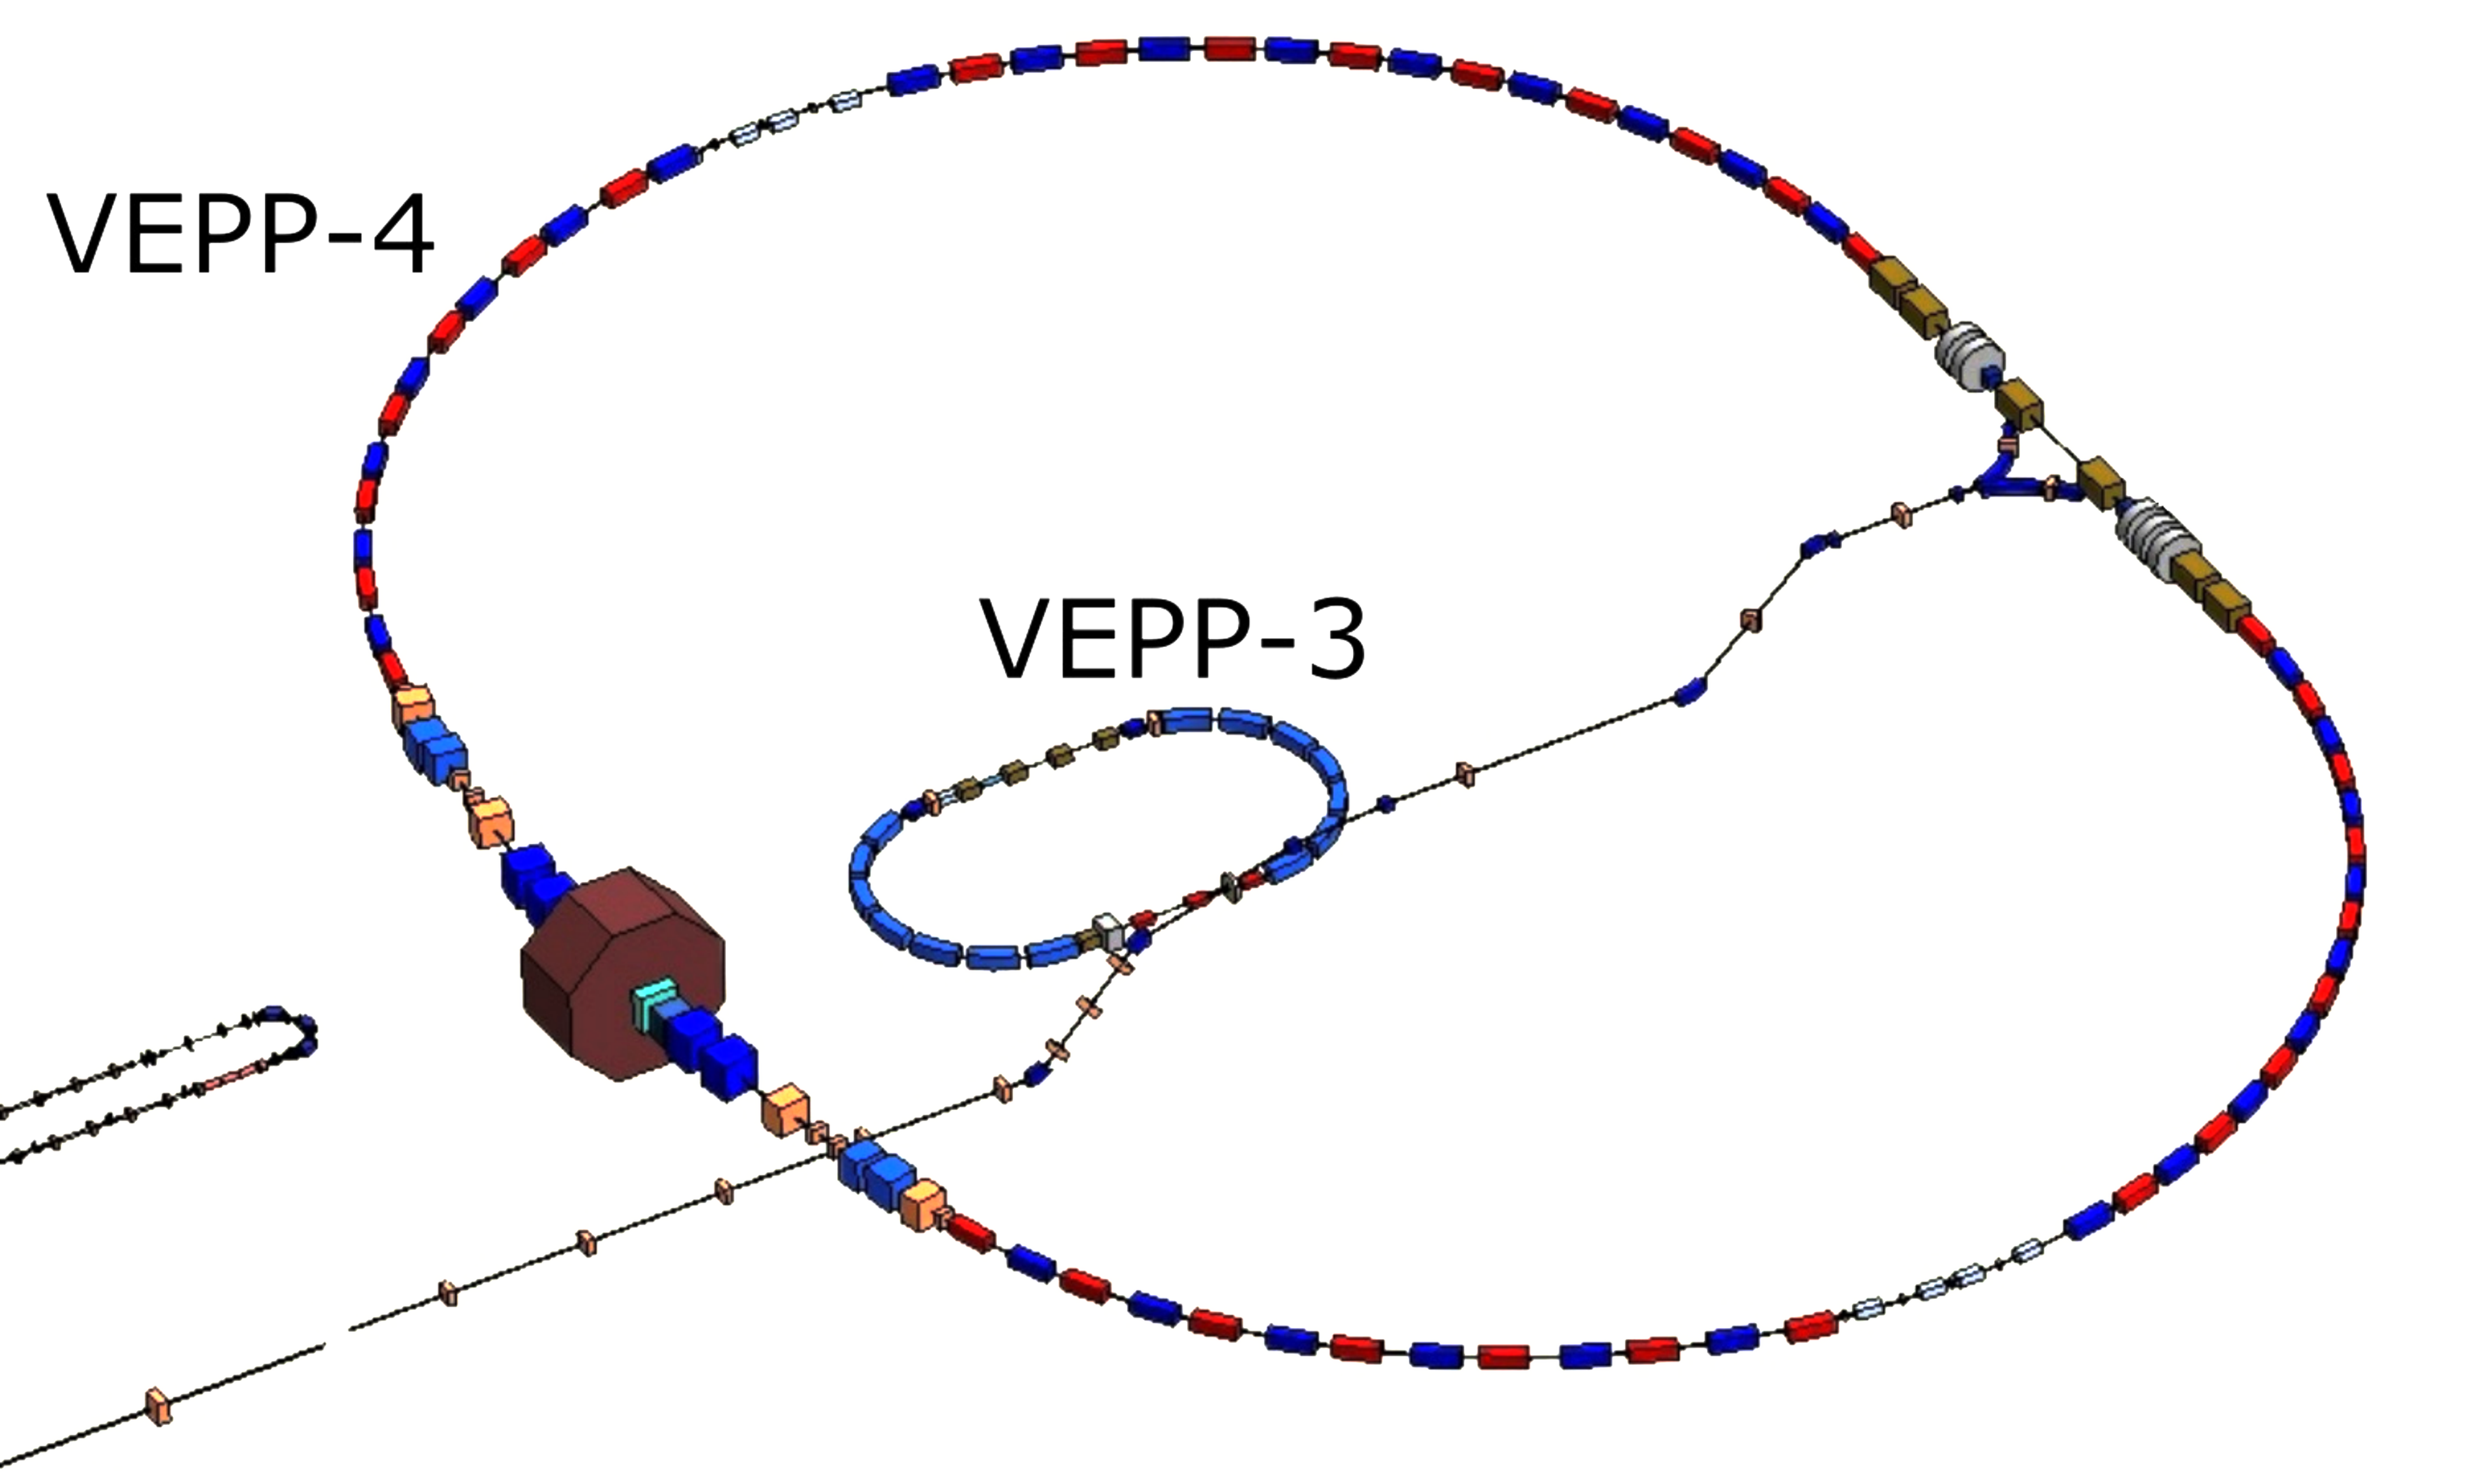
\includegraphics[width=1\linewidth]{VEPP-4.pdf}
			\footnotesize{Коллайдер ВЭПП-4М}
			\end{center}
		\end{minipage}
		\begin{minipage}[h]{0.49\linewidth}
			\begin{center}
				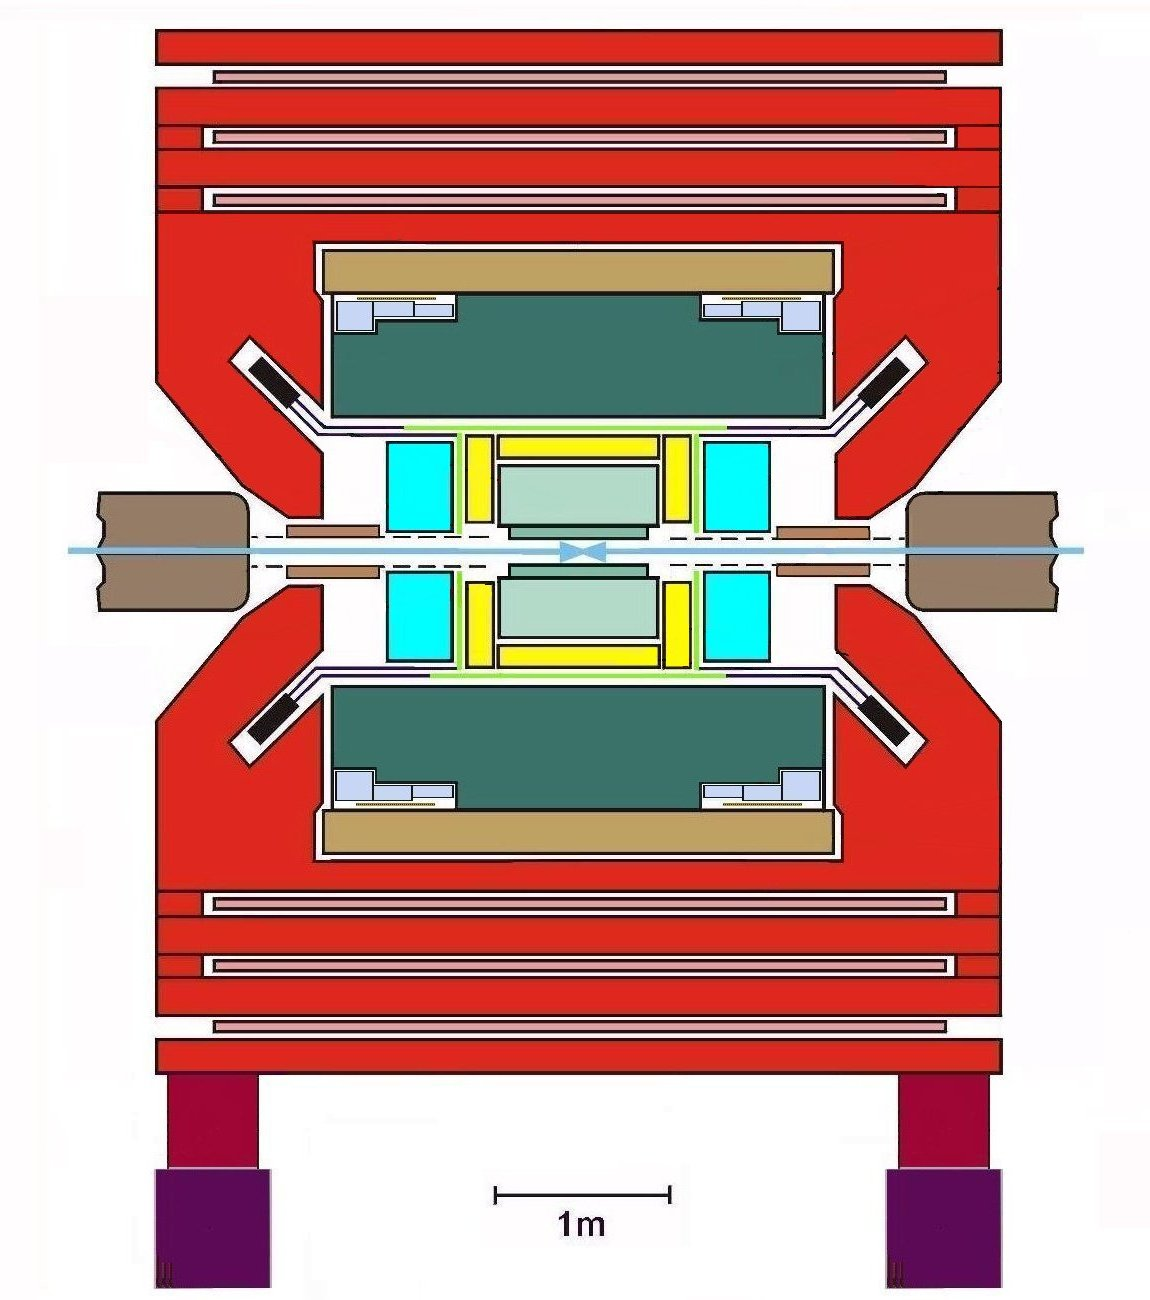
\includegraphics[width=0.6\linewidth]{KEDR.jpg}\\
				\footnotesize{Детектор КЕДР}
			\end{center}
				
		\end{minipage}
	\begin{center}
		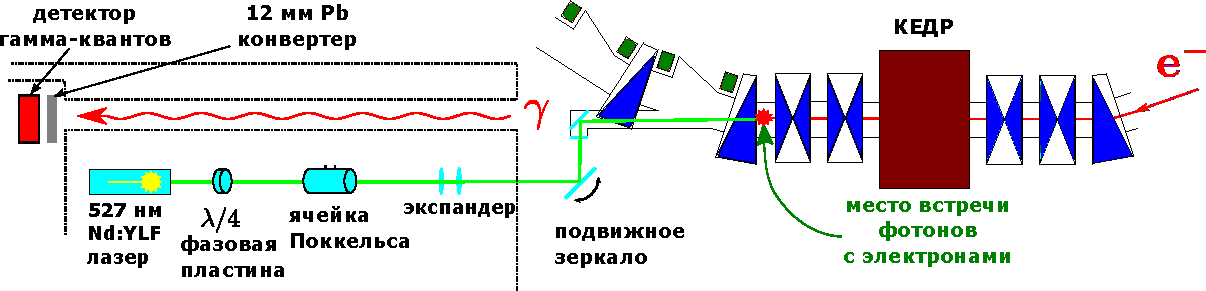
\includegraphics[width=0.8\linewidth]{LSRP_scheme.pdf}\\
		\footnotesize{Лазерный поляриметр}
	\end{center}
\end{frame}

\begin{frame}
\frametitle{Метод резонансной деполяризации}
	\vspace{30pt}
	\begin{columns}
		\column{0.4\textwidth}
		\begin{minipage}[t][1\textheight]{\linewidth}
				\small{\flushleft	Впервые реализован в ИЯФ~СO~РАН в 1974 г. 
				\begin{itemize}
					\item $\Delta E/E \geqslant 10^{-6}$
					\item $\Omega = \omega_s \biggl(1+ \gamma \cfrac{\mu'}{\mu}\biggr)$
					\item Условие резонанса: $\omega_d \pm k \omega_s = \Omega$
					\item Измеряем: $\Delta y = \cfrac{\omega_0}{2m_e}PL\Delta V$
				\end{itemize}}
		\end{minipage}%
		\column{0.6\linewidth}
		\begin{minipage}[t][1\textheight]{\linewidth}
			\begin{picture}(10,10)(0,120)
				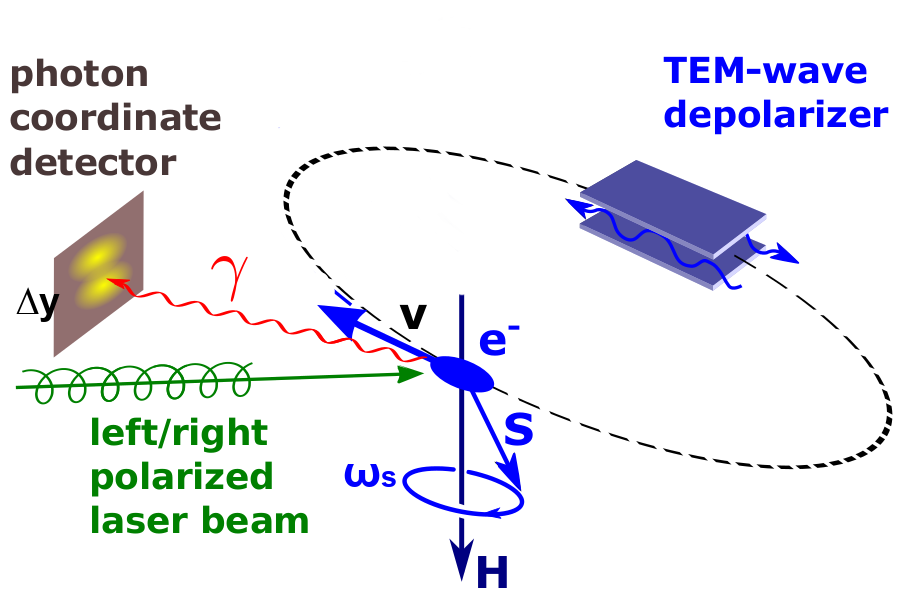
\includegraphics[width=1\linewidth]{mrd-lsrp.png}
			\end{picture}
		\end{minipage}%
	\end{columns}
	\begin{center}
		
	\end{center}
\end{frame}

\begin{frame}
	\frametitle{Мотивация}
	\begin{minipage}[h]{0.55\linewidth}
	\small{
	\begin{itemize}
		\item Прецизионные измерения масс в области $\Upsilon-\text{резонанса}$
		~($m = 9.46~\GeVovercsq$) 
		\item Использование метода резонансной деполяризации при измерении энергии пучков
		\item Создание установки <<Лазерный поляриметр>>
		\item \textbf{Необходим координатный детектор гамма-квантов}
	\end{itemize}}
	\hfill
	\end{minipage}
		\begin{minipage}[h]{0.43\linewidth}
			\includegraphics[width=1\linewidth]{UpsilonMass.png}
			\\\tiny{Рисунок из статьи: A.S. Artamonov \emph{et al.}, High Precision Measurement of the Y Meson Mass, 1982}
		\end{minipage}
	\end{frame}

\begin{frame}
\frametitle{Цель}
Создание прототипа GEM-детектора для установки <<Лазерный поляриметр>> и исследование его физических характеристик
\end{frame}

\begin{frame}[t]
\frametitle{Задачи}
	\begin{itemize}
		\item Изучение физических принципов работы газовых электронных умножителей
		\item Создание детектора на основе GEM 
		\item Определение его физических характеристик:
		\begin{itemize}
			\item уровня шумов
			\item коэффициента усиления
			\item пространственного разрешения
			\item эффективности регистрации
		\end{itemize}
	\end{itemize}
\end{frame}

\begin{frame}
\frametitle{Газовые электронные умножители (GEM)}
\begin{center}
	\begin{minipage}[h]{0.49\linewidth}
		\includegraphics[width=1\linewidth]{GEM_microphoto.png}
	\end{minipage}
	\begin{minipage}[h]{0.49\linewidth}
		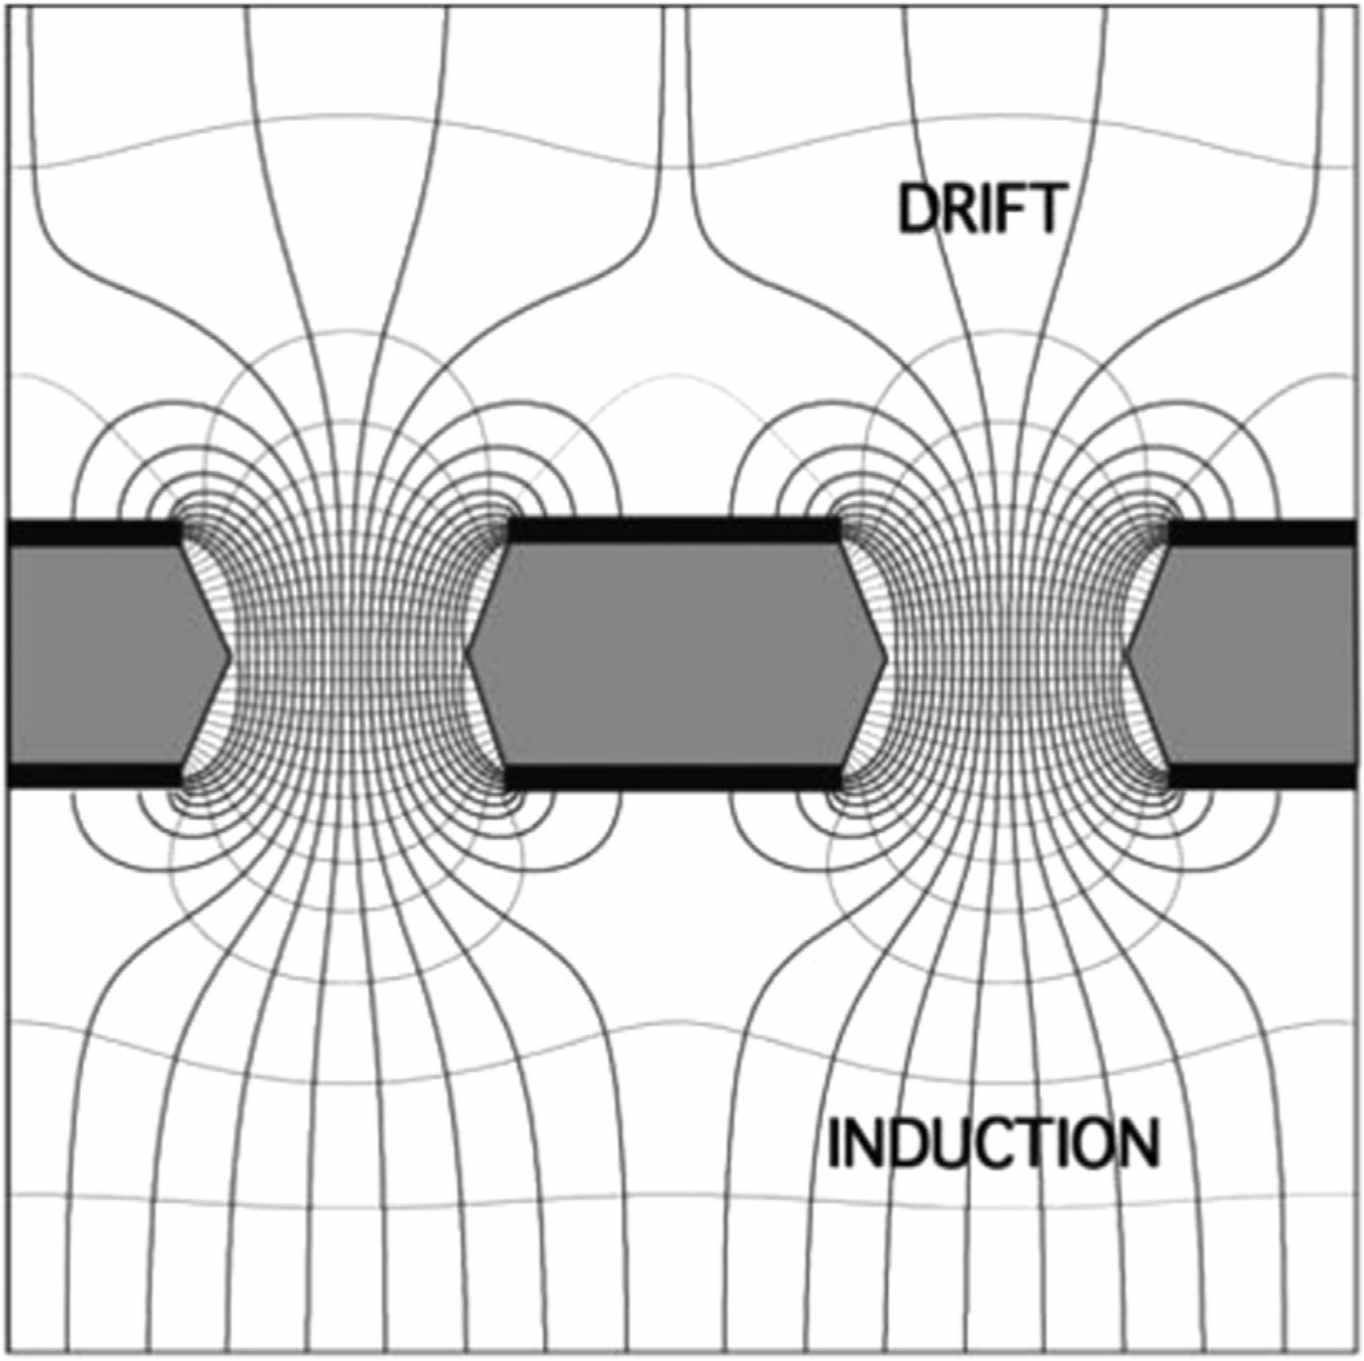
\includegraphics[width=1\linewidth]{GEM_crossec.jpg}
	\end{minipage}
	\tiny{Рисунки из статьи: F. Sauli, The gas electron multiplier (GEM): Operating principles and applications, 2016}
	
\end{center}
\end{frame}

\begin{frame}[t]
\frametitle{Принцип работы GEM детектора}
\vspace{0pt}
\begin{columns}
\column{0.5\textwidth}
\begin{minipage}[t][1\textheight]{\linewidth}
	\small{\begin{itemize}
			\item Первичная частица $\Rightarrow$ $e^-$ ионизации
			\item Дрейф $e^-$ в область с высоким полем
			\item Возникновение электронных лавин в отверстиях GEM
			\item Проникновение $e^-$ в индукционный промежуток
			\item Регистрация заряда считывающей структурой
	\end{itemize}}
\end{minipage}%
\column{0.5\linewidth}
\begin{minipage}[t][1\textheight]{\linewidth}
	\center 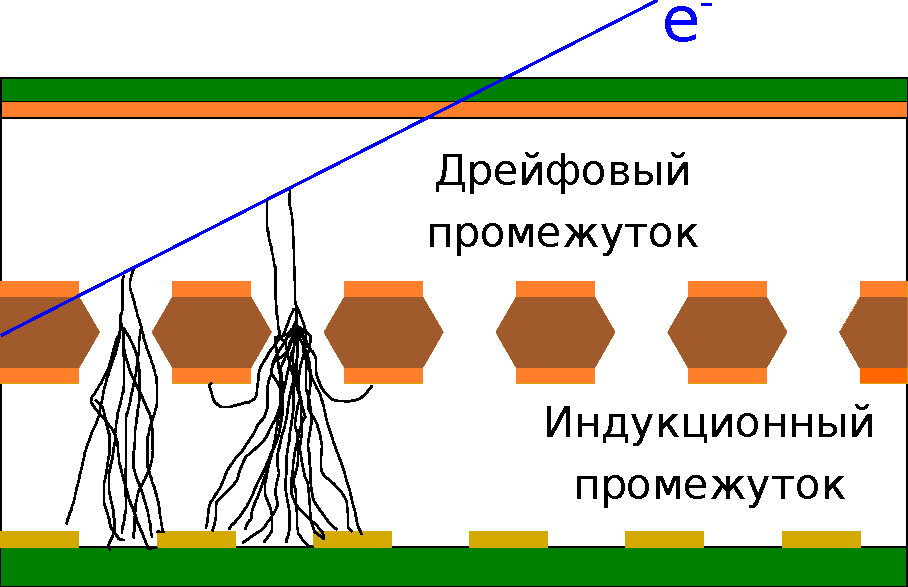
\includegraphics[width=0.9\linewidth]{GEM_scheme.pdf}
	\vspace*{0pt}
	\center 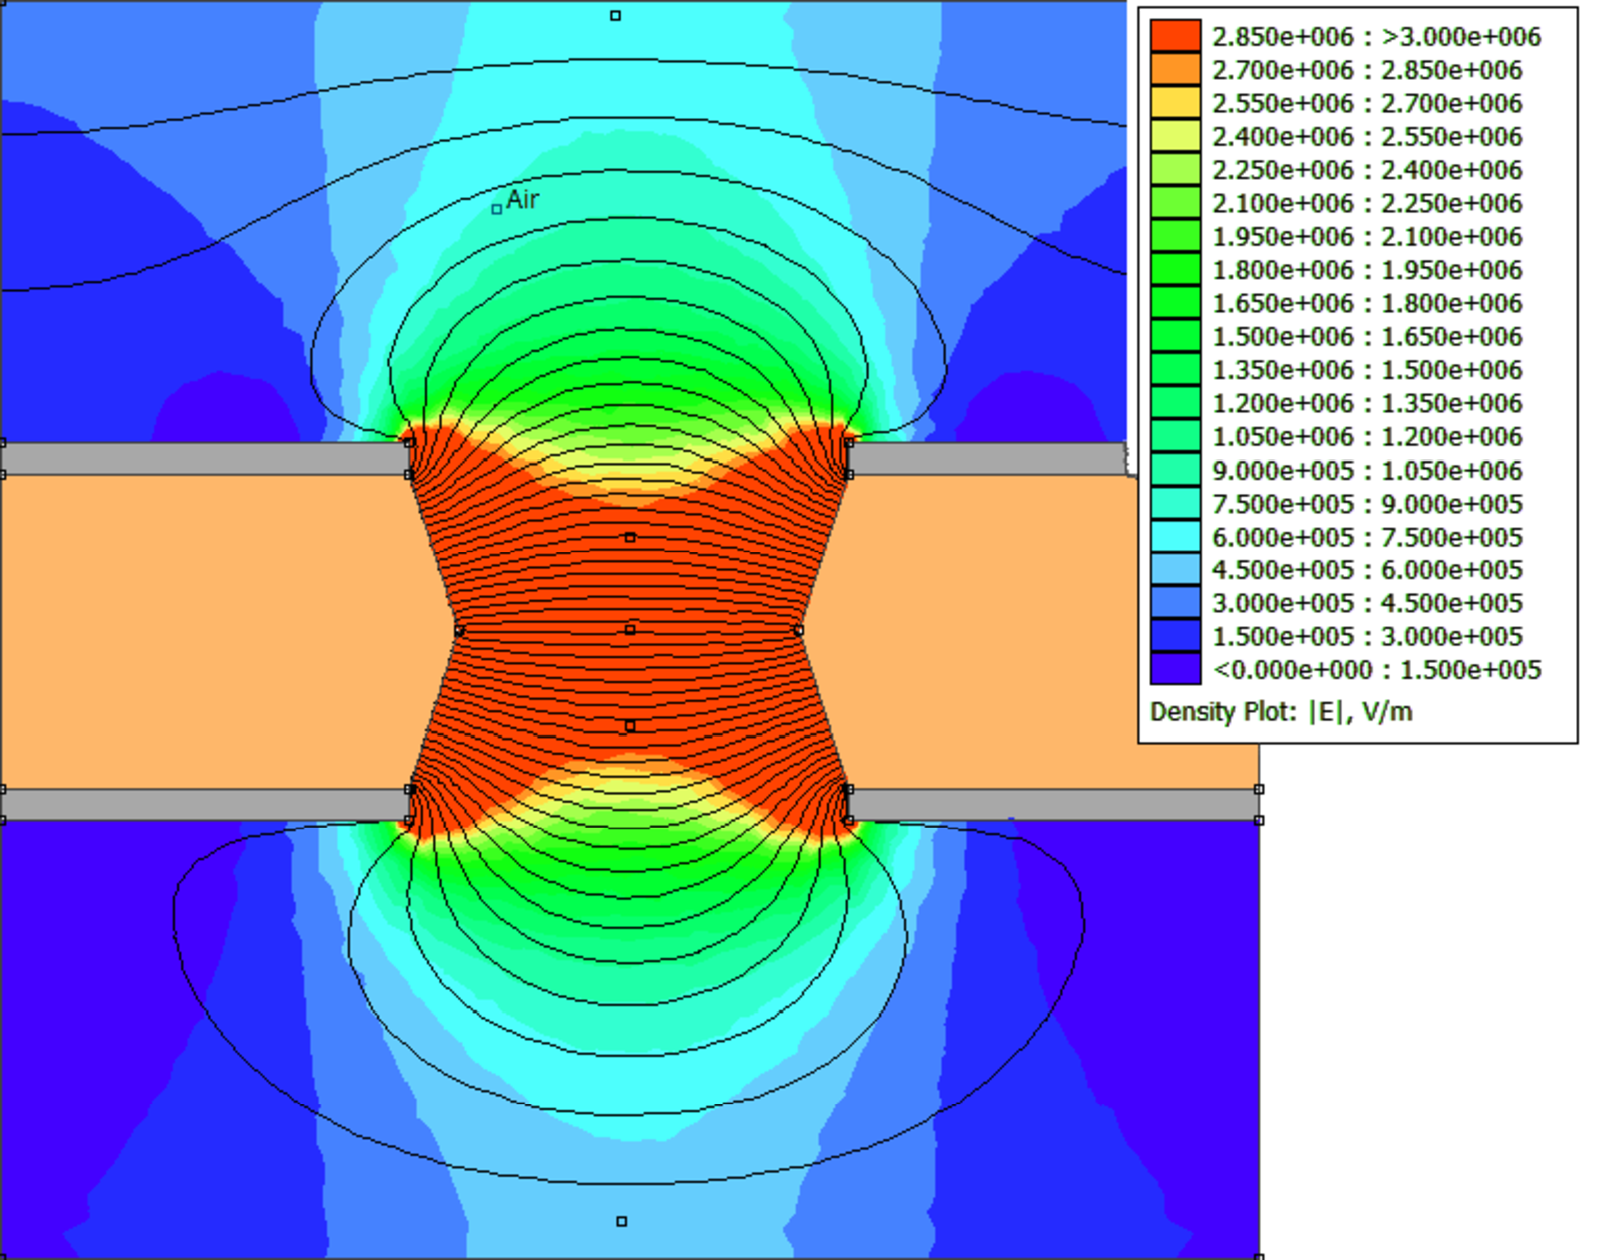
\includegraphics[width=0.6\linewidth]{GEM_field.pdf}	
\end{minipage}%
\end{columns}
\end{frame}

\begin{frame}[t]
\frametitle{Ключевые параметры детектора для лазерного поляриметра}
		\begin{itemize}
				\item \textit{Уровень шумов:} шумы АЦП, кросс-токи, сторонние наводки
				\item  \textit{Коэффициент усиления:} напряжение на GEM, геометрия усиливающей структуры
				\item  \textit{Пространственное разрешение:} геометрия считывающей структуры 
		\end{itemize}
\end{frame}


\begin{frame}[t]
\frametitle{Прототип детектора}
		\begin{minipage}[c]{0.59\linewidth}
			\centering
			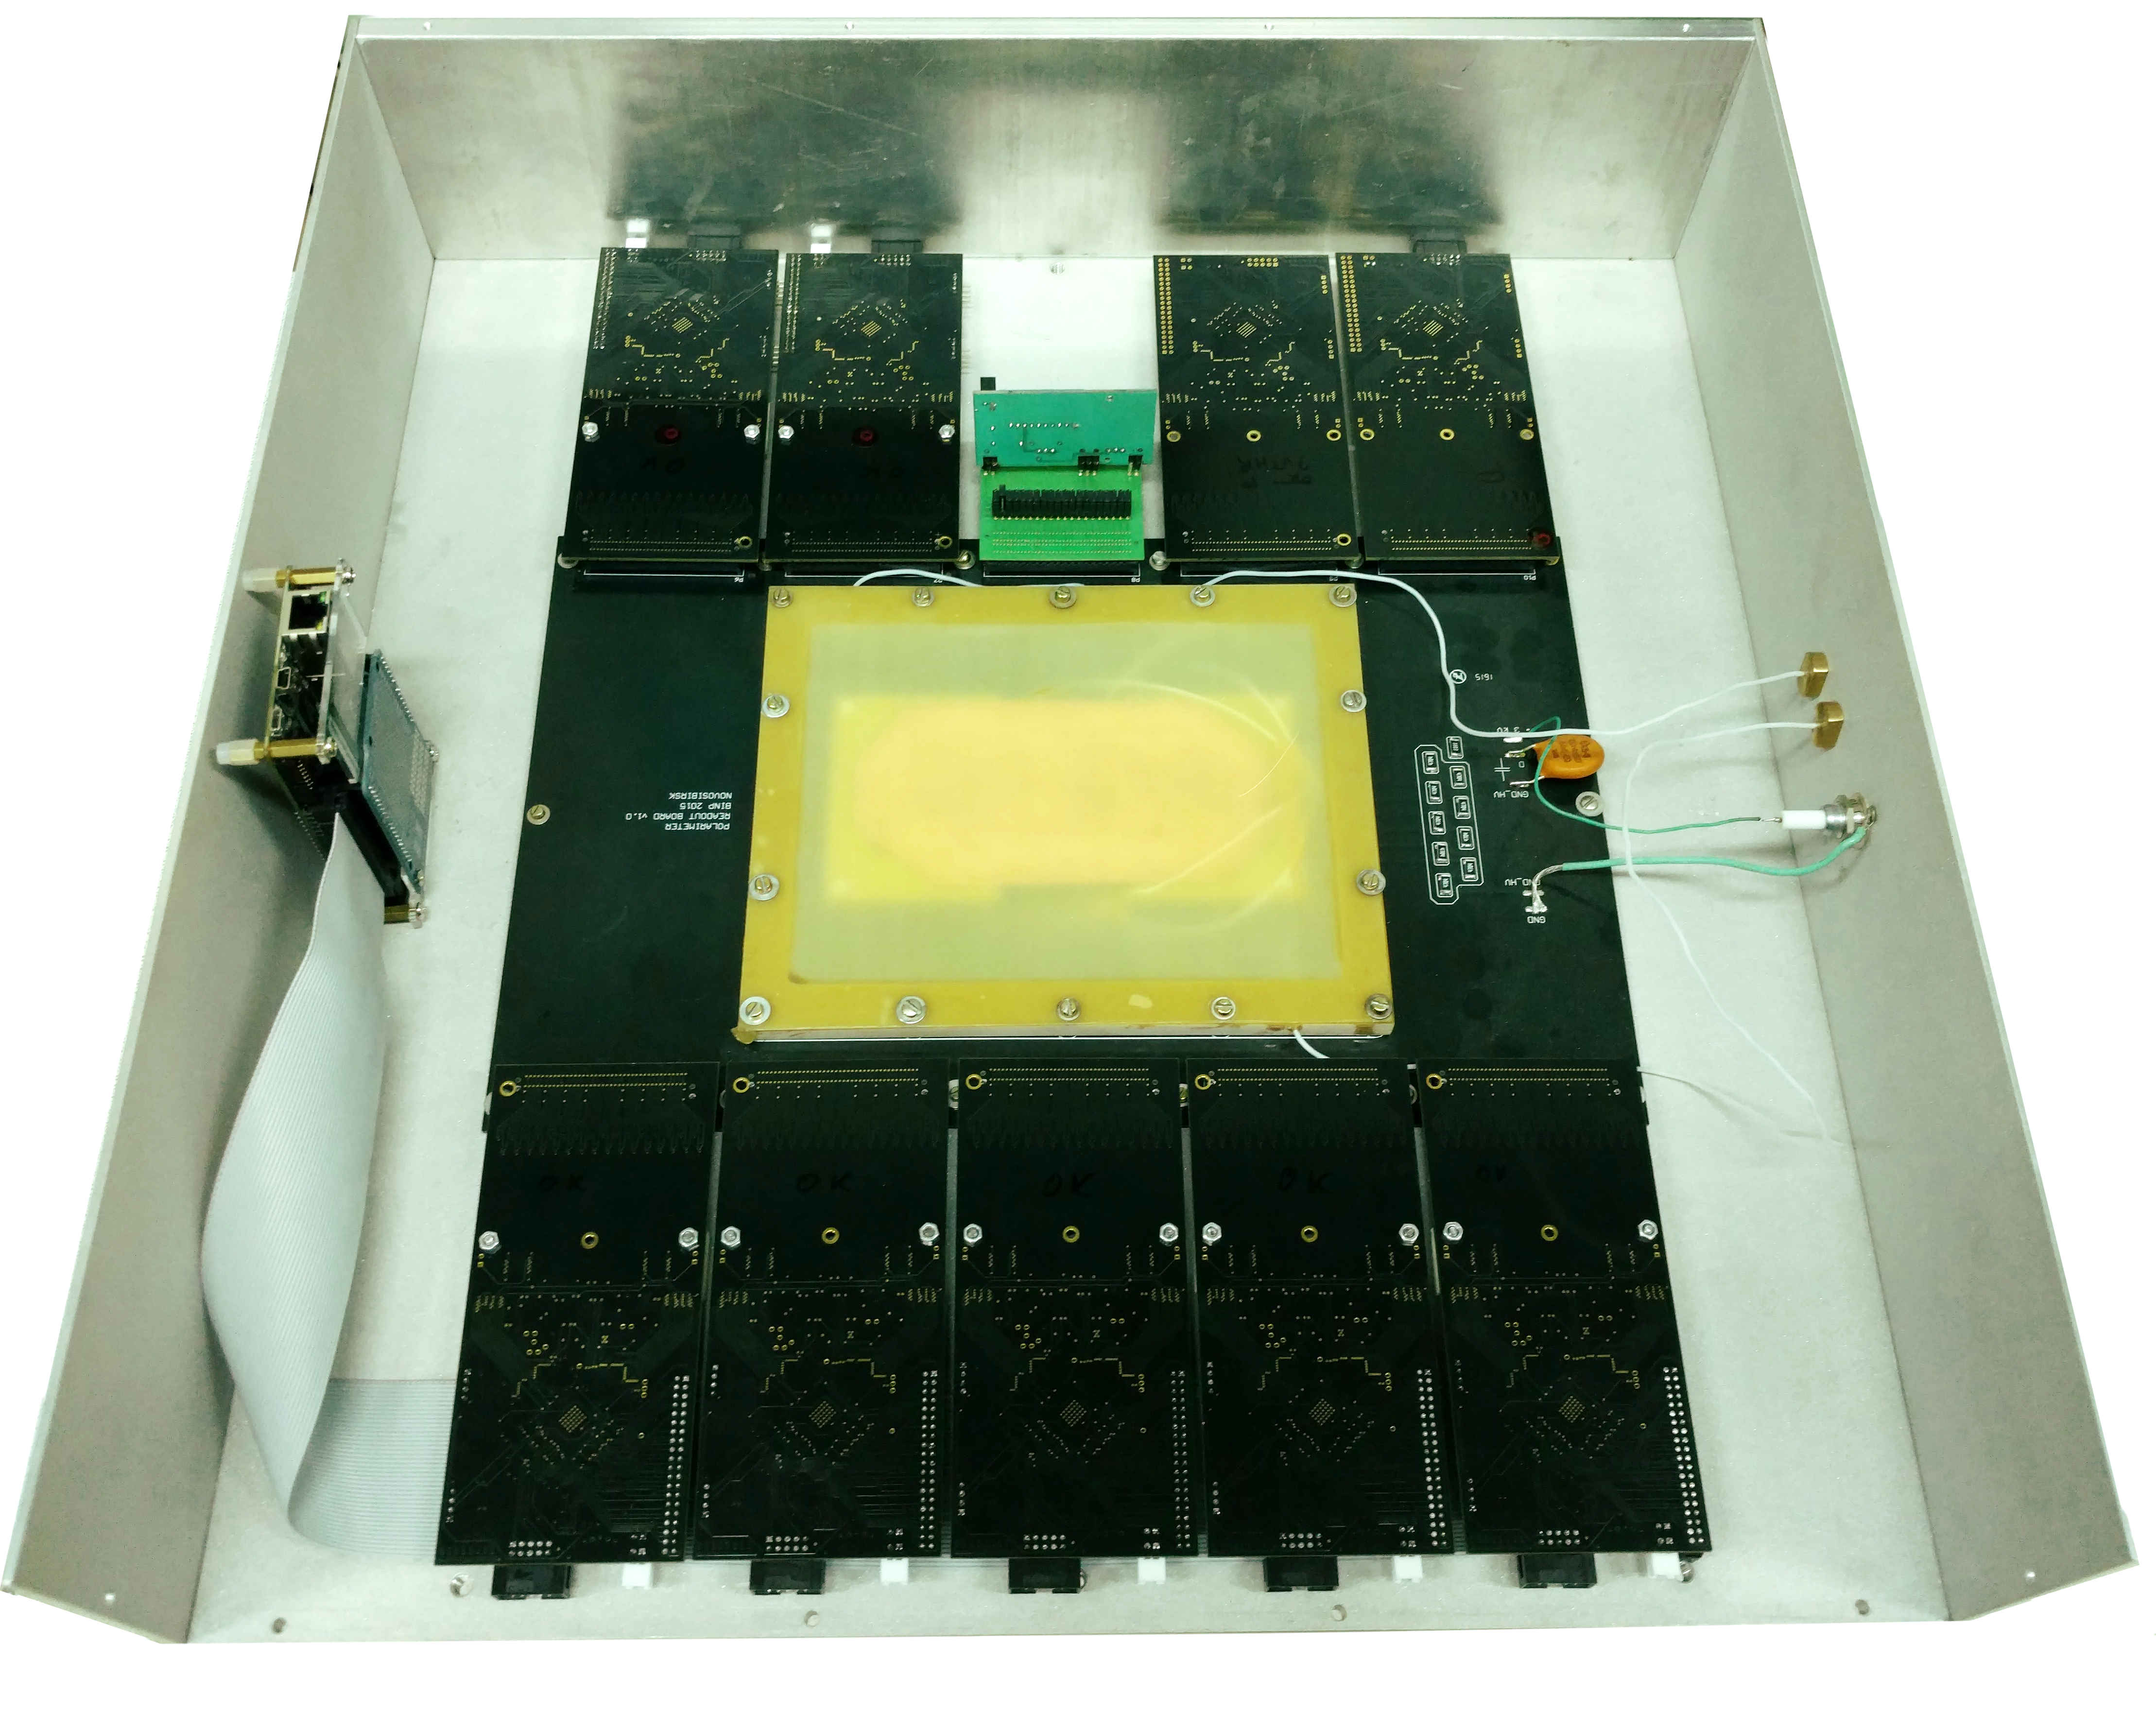
\includegraphics[width=1\linewidth]{GEM_prototype.jpg} 
			\newline \tiny{Детектор в сборе}
		\end{minipage}
		\begin{minipage}[t]{0.39\linewidth}
		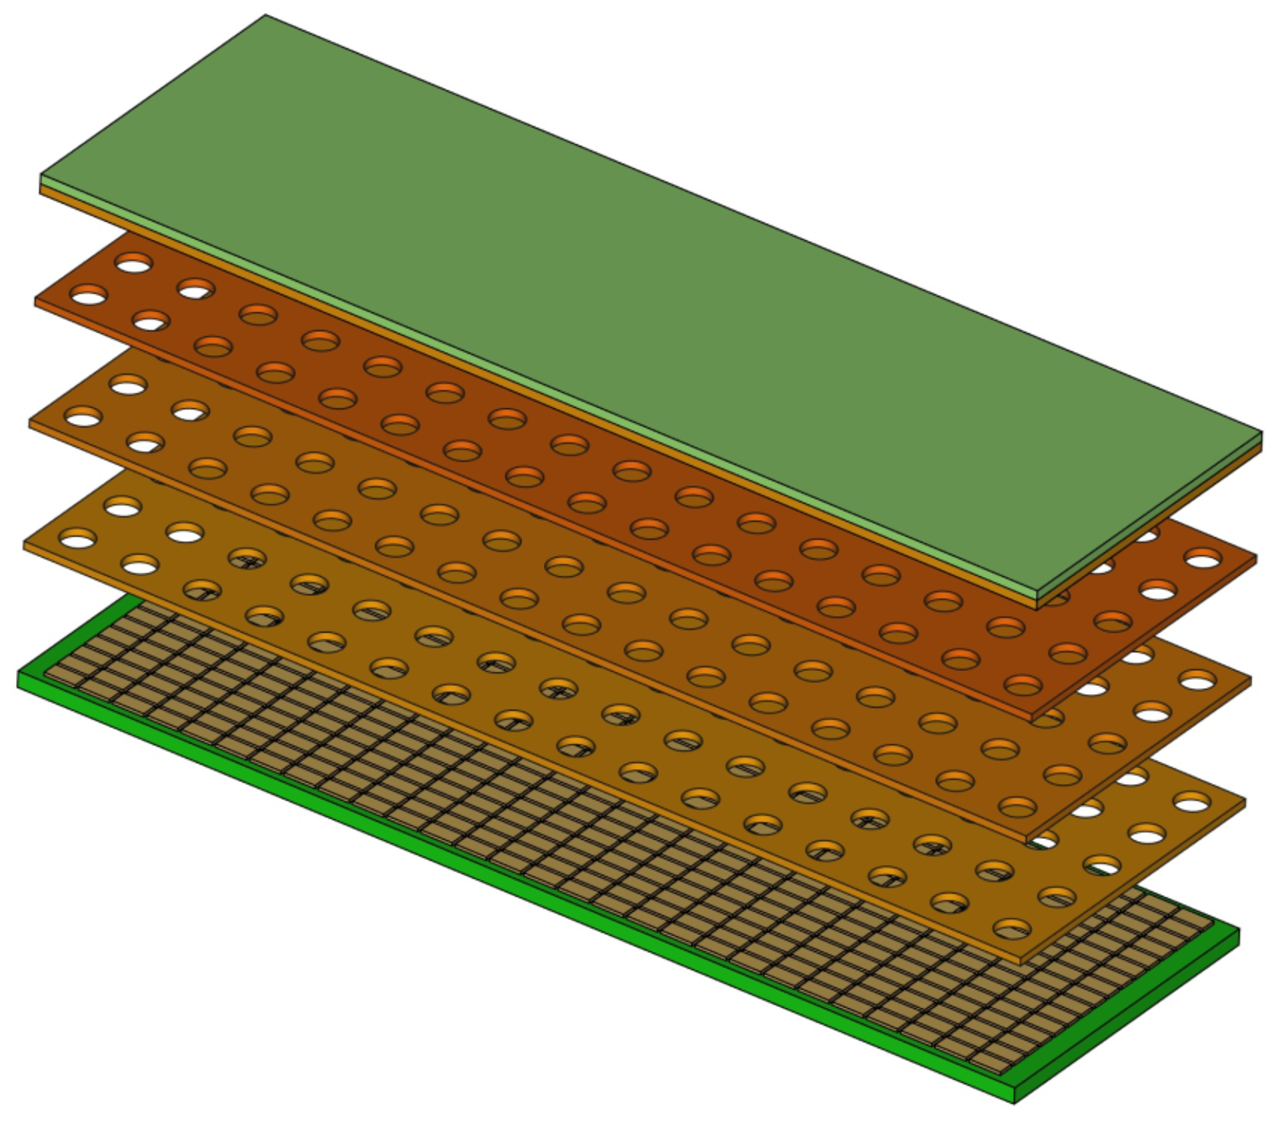
\includegraphics[width=1\linewidth, height = 0.4\textheight]{GEM_model.pdf}
		\tiny{Расположение электродов и считывающей структуры}
		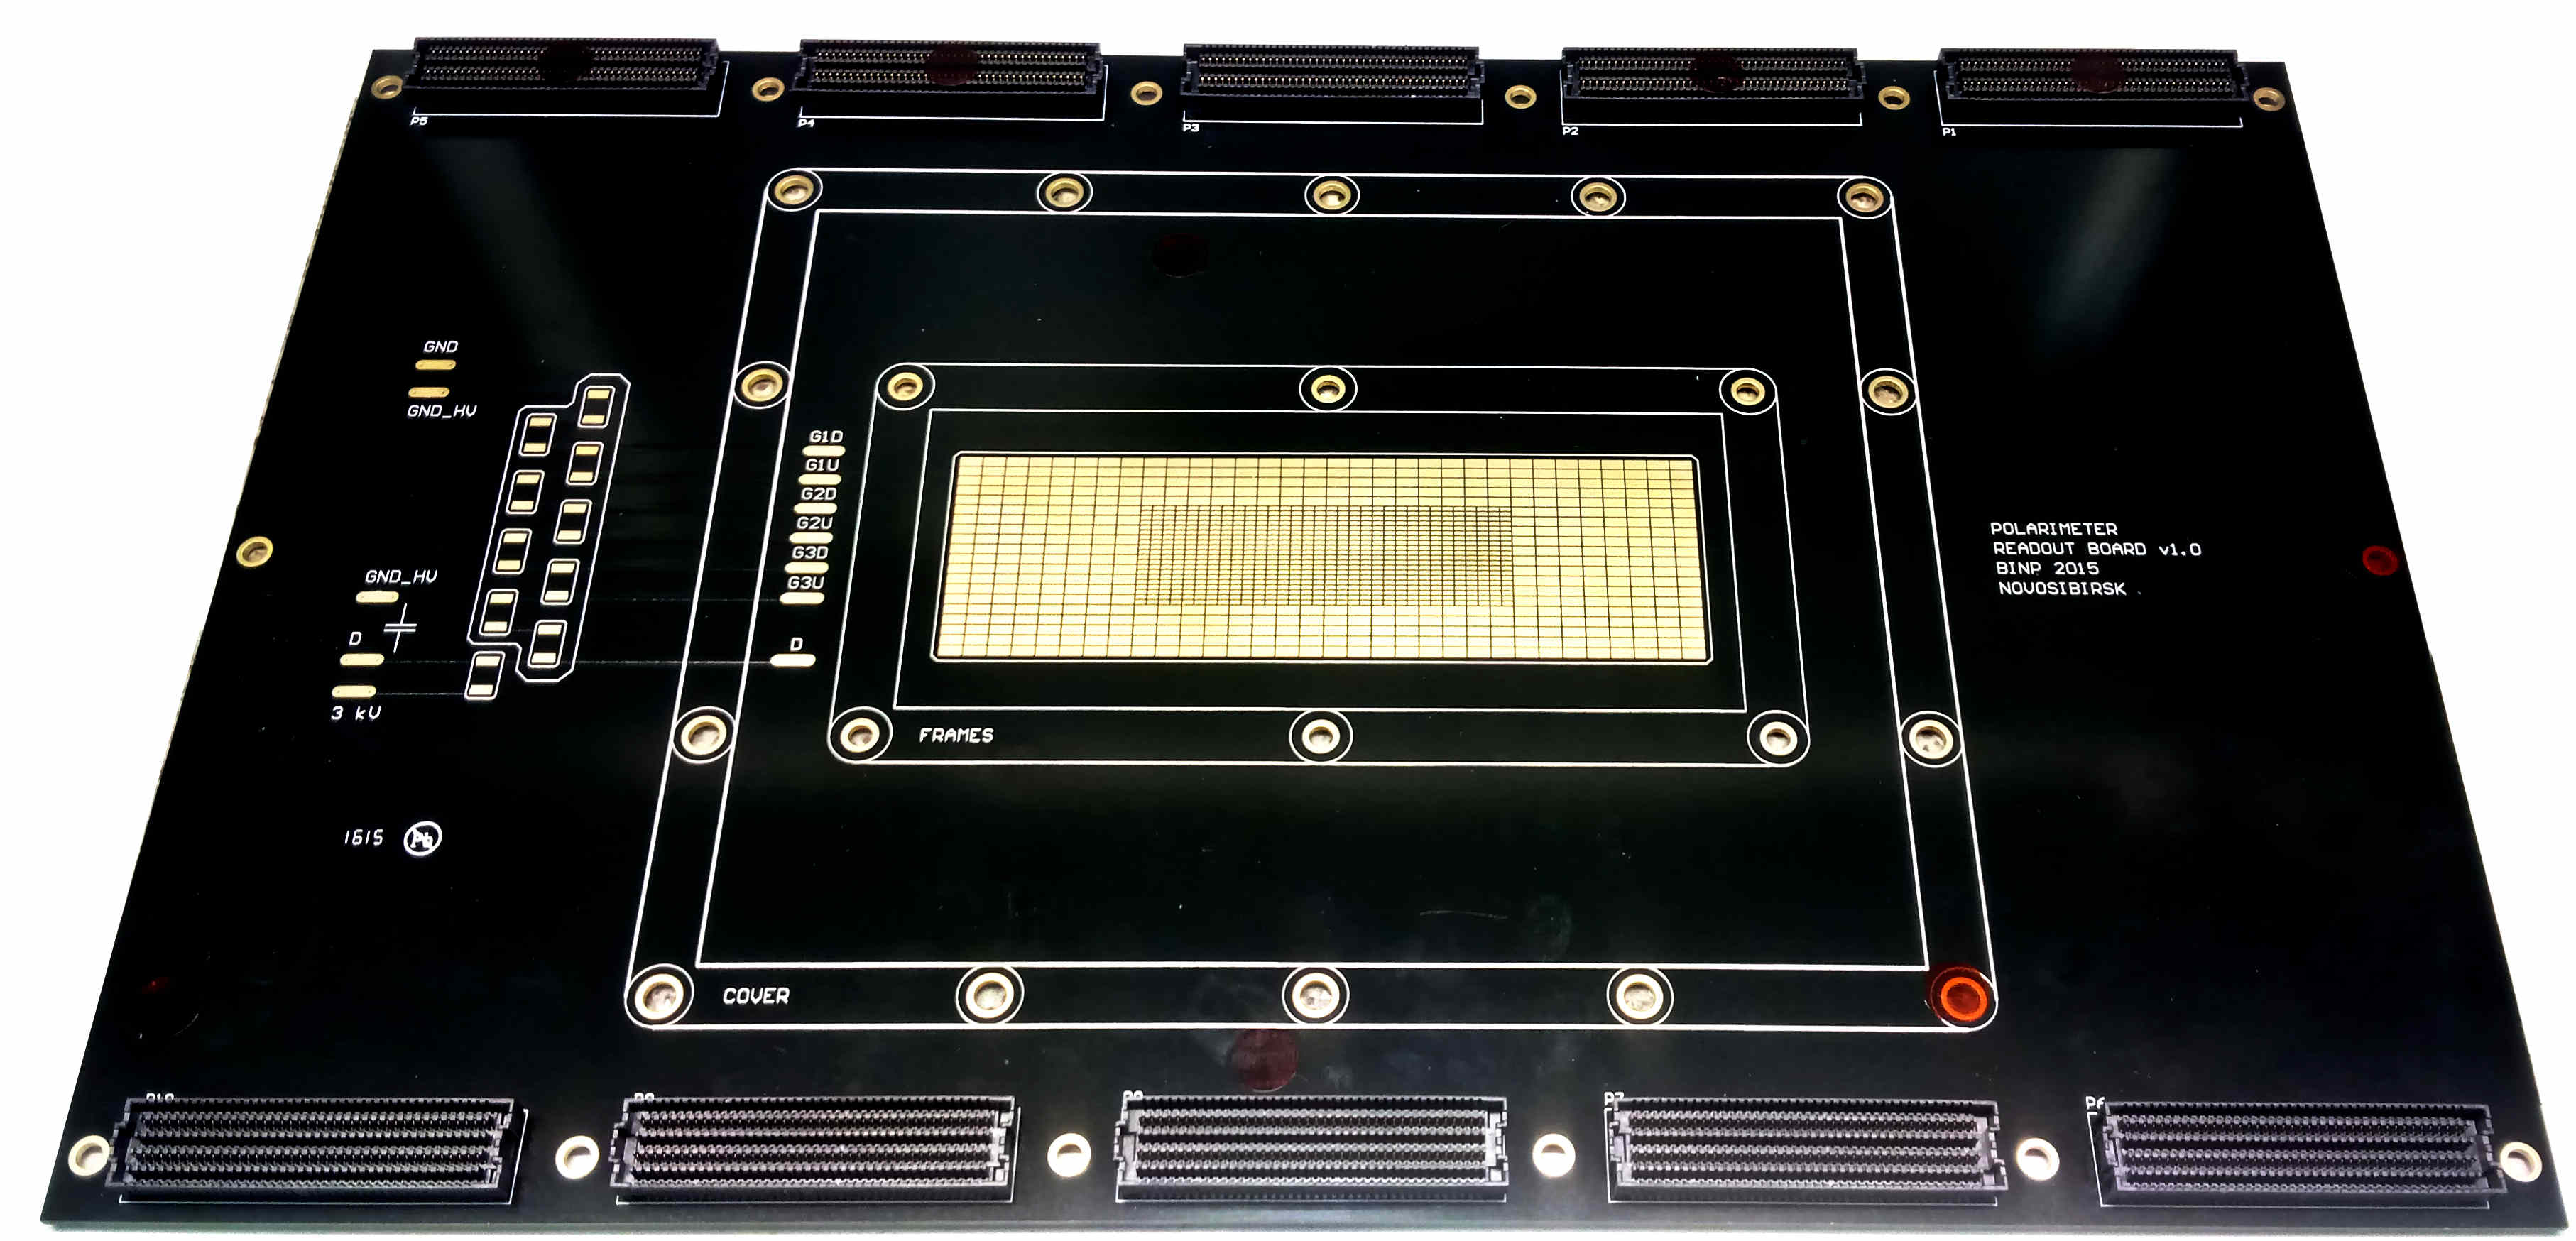
\includegraphics[width=1\linewidth]{Main_board.jpg} 
		\newline \centering\tiny{Главная плата}
		\end{minipage}	
\end{frame}

\begin{frame}[c]
\frametitle{Определение уровня шумов детектора}
	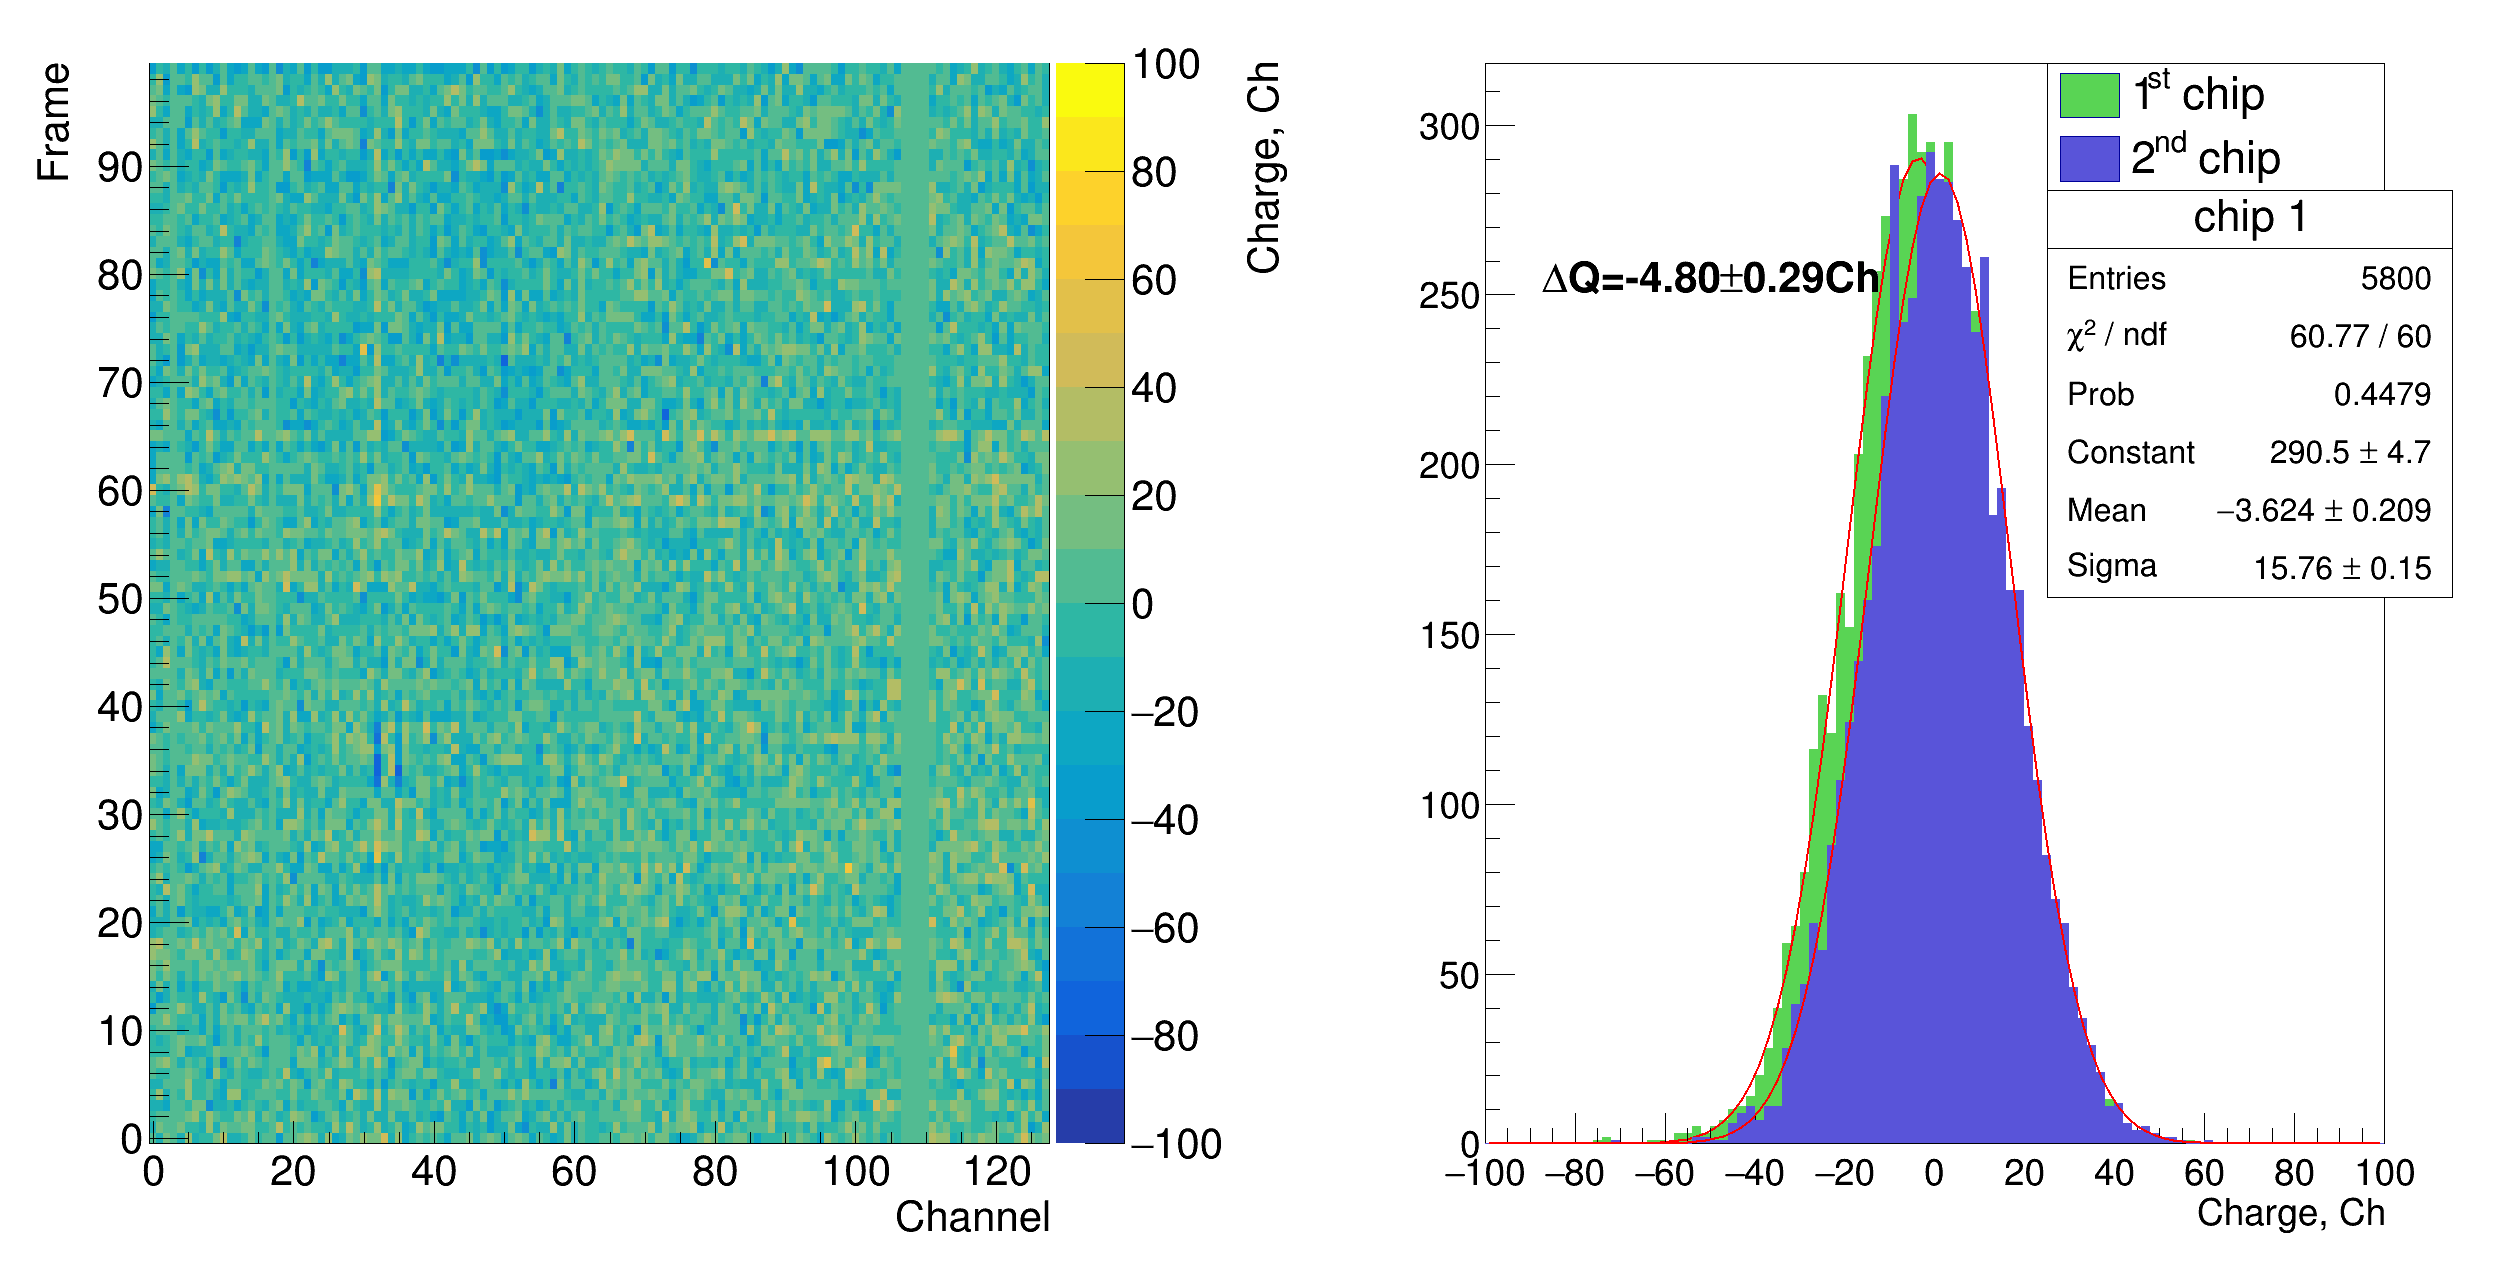
\includegraphics[width=1\linewidth]{Noise_no_filtering.png}
	 \hspace*{20pt}\tiny{0--59 --- Чип 1}\hspace*{30pt}\tiny{68--127 --- Чип 2}
\end{frame}

\begin{frame}[c]
\frametitle{Первичные наблюдения}
\vspace{10pt}
\begin{columns}
	\column{0.5\textwidth}
	\begin{minipage}[t][1\textheight]{\linewidth}
		\vspace{10pt}
		\small{\begin{itemize}
				\item Наличие шумящих каналов
				\item Cдвиг нулевого уровня у АЦП
				\item Имеют место флуктуации среднего по кадру
				\item Уровень шумов: $\sigma_n \approx 16$~Ch
		\end{itemize}}
	\end{minipage}%
	\column{0.5\linewidth}
	\begin{minipage}[t][1\textheight]{\linewidth}
		\vspace*{8pt}
		\hspace*{5.5pt}
        \includegraphics[width=0.915\linewidth]{Noise_no_filtering_hist.png}
	\end{minipage}
\end{columns}
\end{frame}
\begin{frame}[c]
\frametitle{Измерение уровня шумов}
\vspace{10pt}
\begin{columns}
	\column{0.4\textwidth}
	\begin{minipage}[t][1\textheight]{\linewidth}
		\vspace*{38pt}
		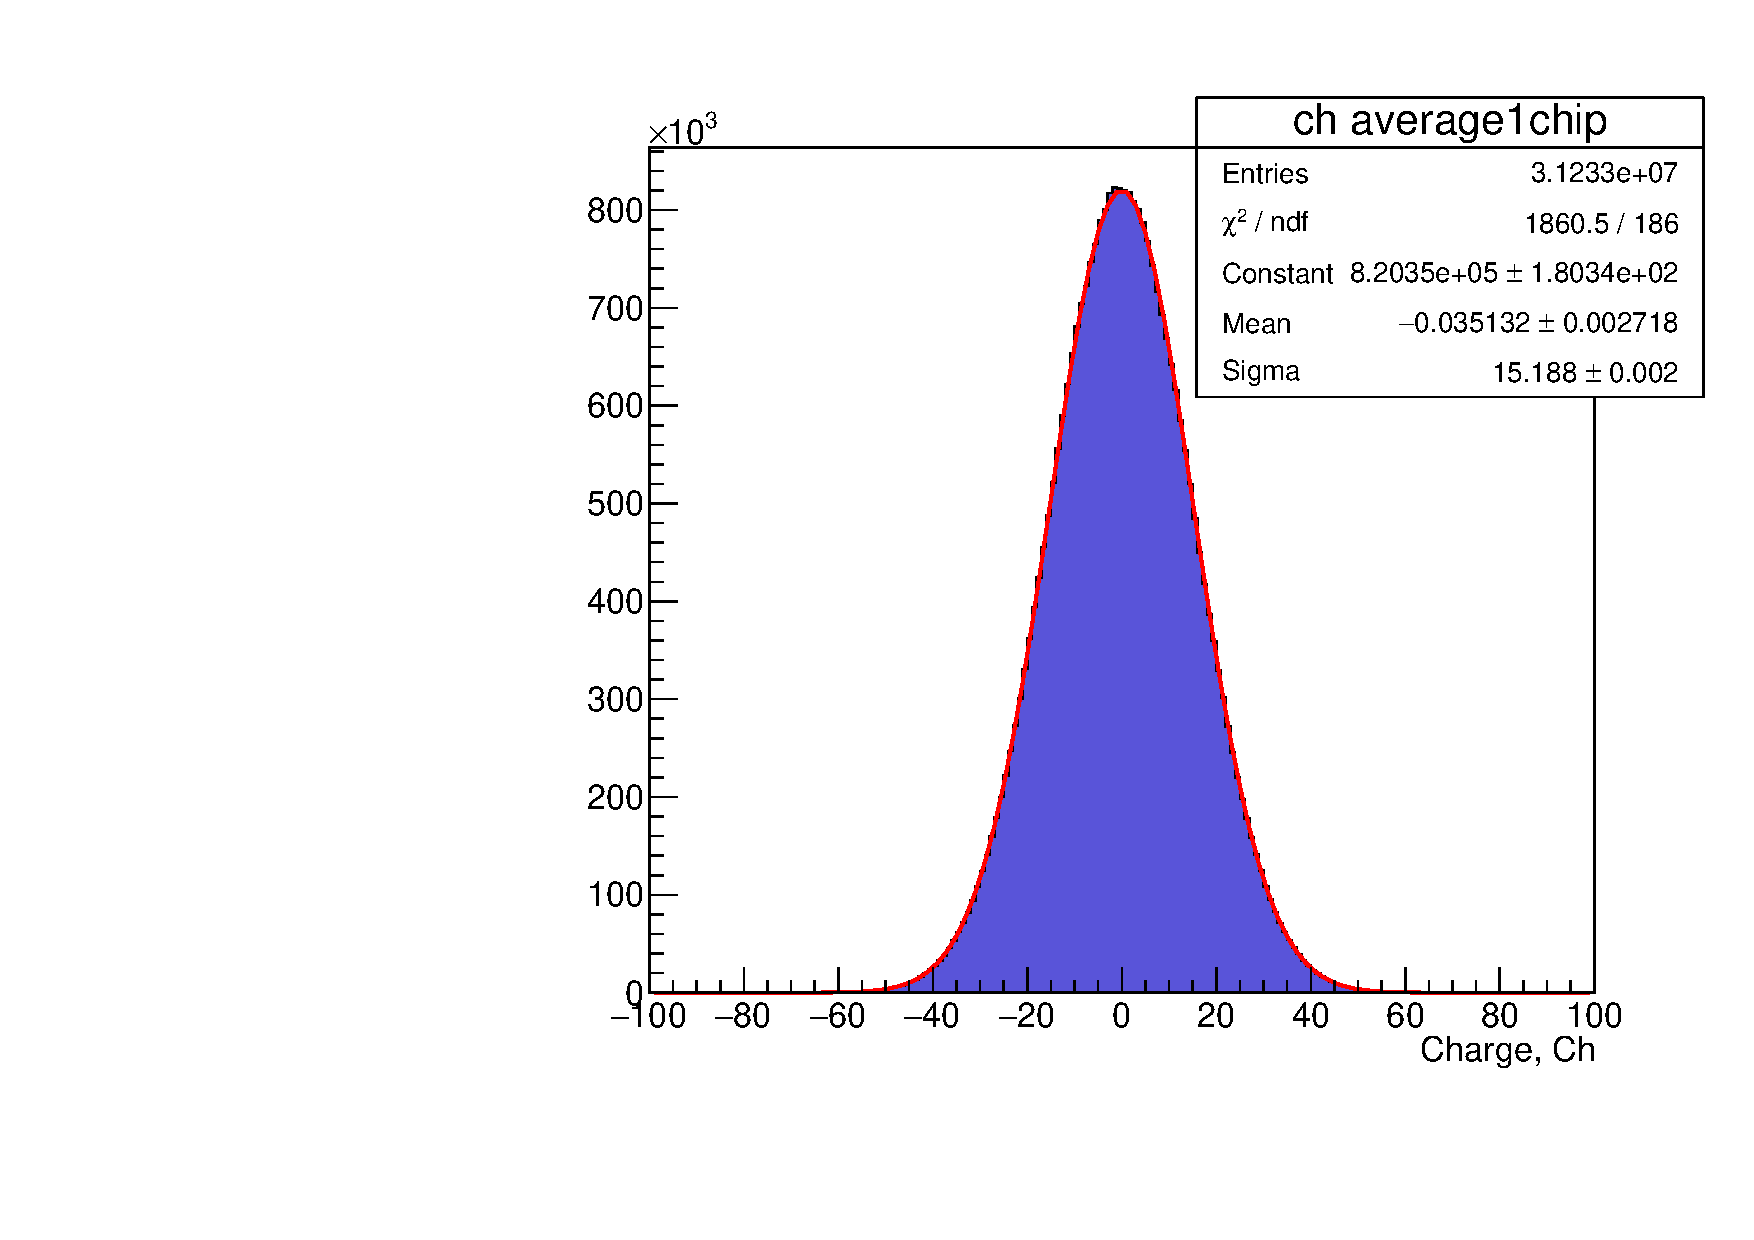
\includegraphics[width=1\linewidth]{Noise_stat.pdf}
	\end{minipage}%
	\column{0.6\linewidth}
	\begin{minipage}[t][1\textheight]{\linewidth}
	\vspace*{30pt}
	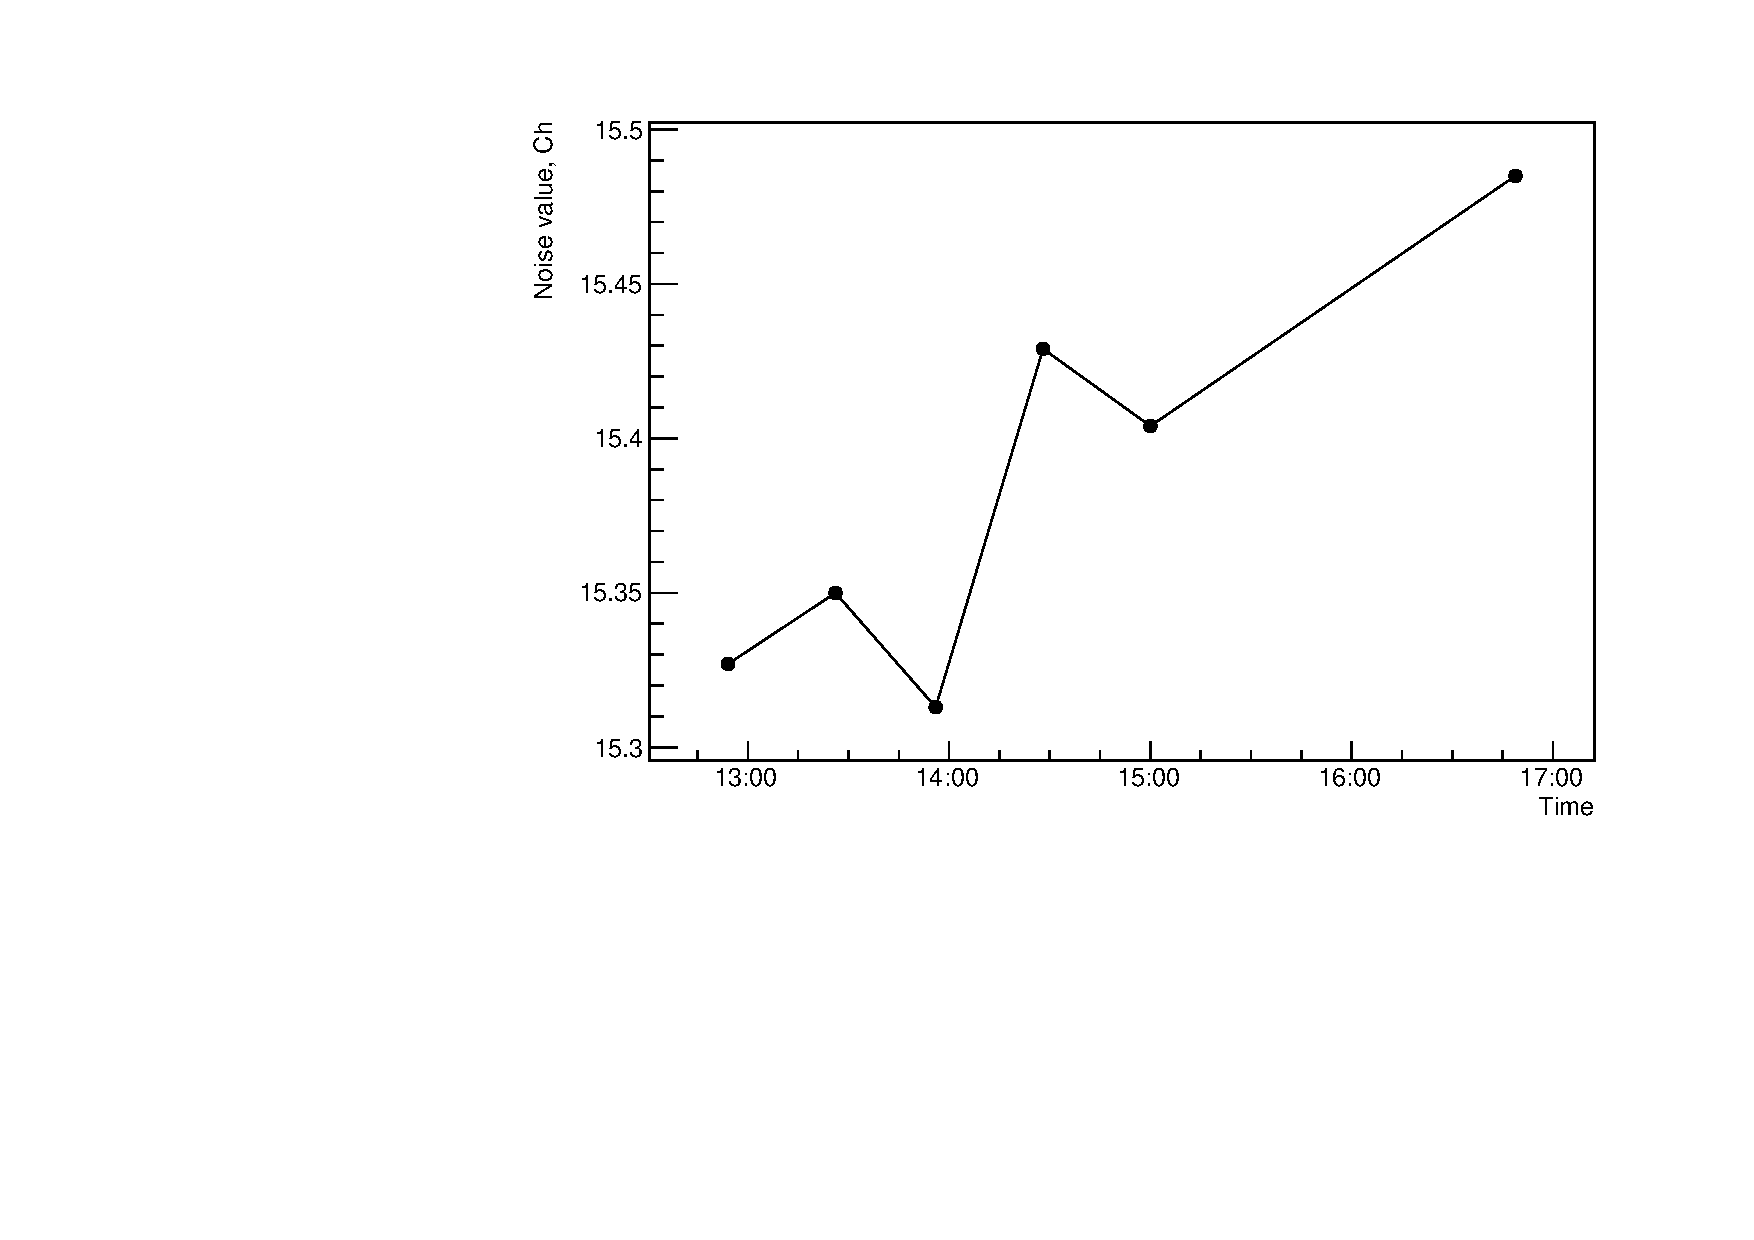
\includegraphics[width=1\linewidth]{Noise_time_drift.pdf}
	\\ \centering \small{$\sigma_{n} \approx 15.4 Ch = 5700 e^{-}$}
	\end{minipage}
\end{columns}
\end{frame}

\begin{frame}[c]
\frametitle{Возможное объяснение: температурный дрейф}
\vspace{10pt}
\begin{columns}
	\column{0.5\textwidth}
	\begin{minipage}[t][1\textheight]{\linewidth}
		\centering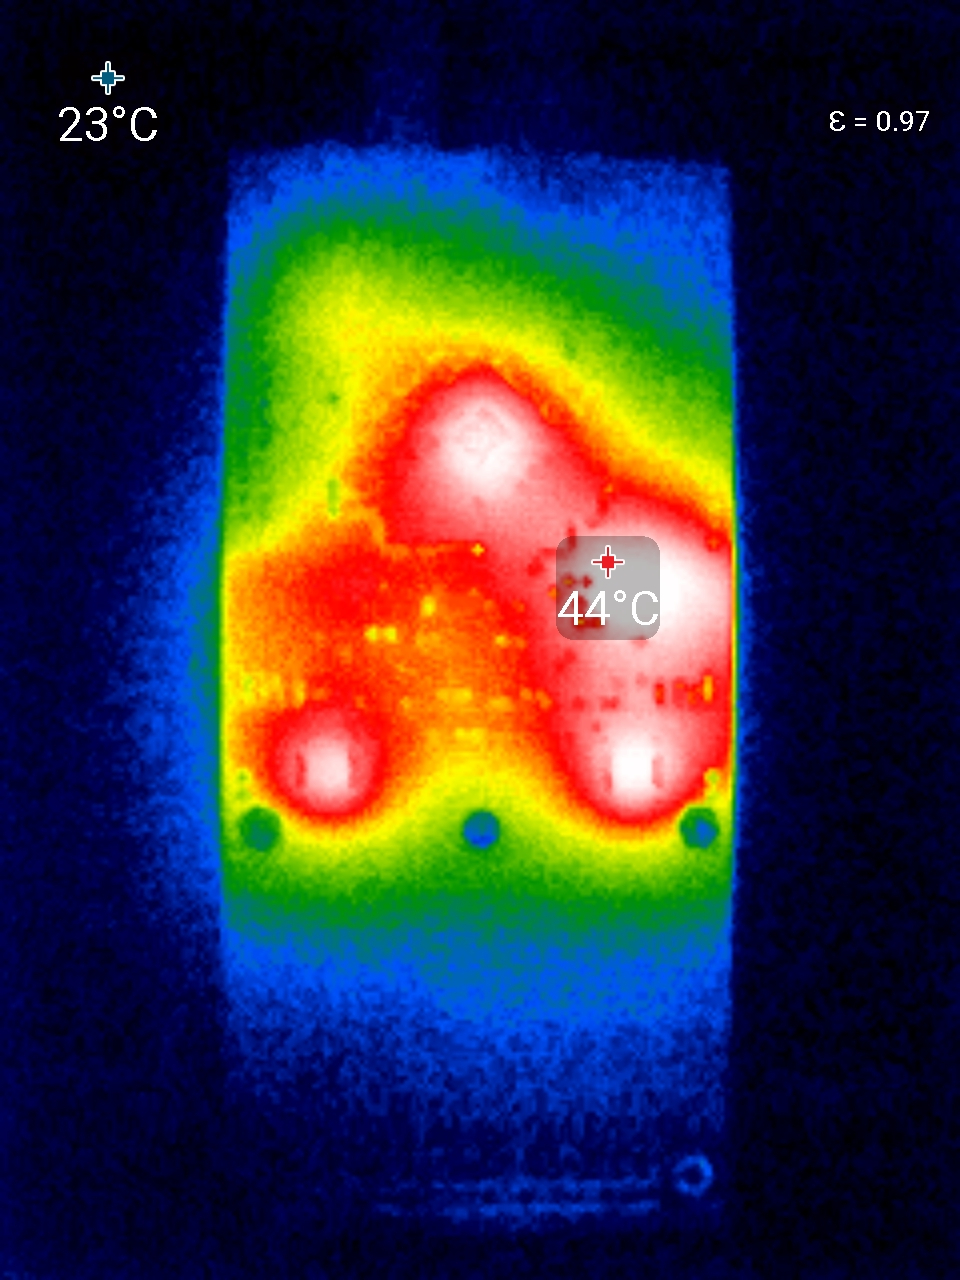
\includegraphics[width=0.8\linewidth]{Thermal_image.jpg}
		\newline \tiny{Автор фото: Василий Кудрявцев}
	\end{minipage}%
	\column{0.5\linewidth}
	\begin{minipage}[t][1\textheight]{\linewidth}
		\centering 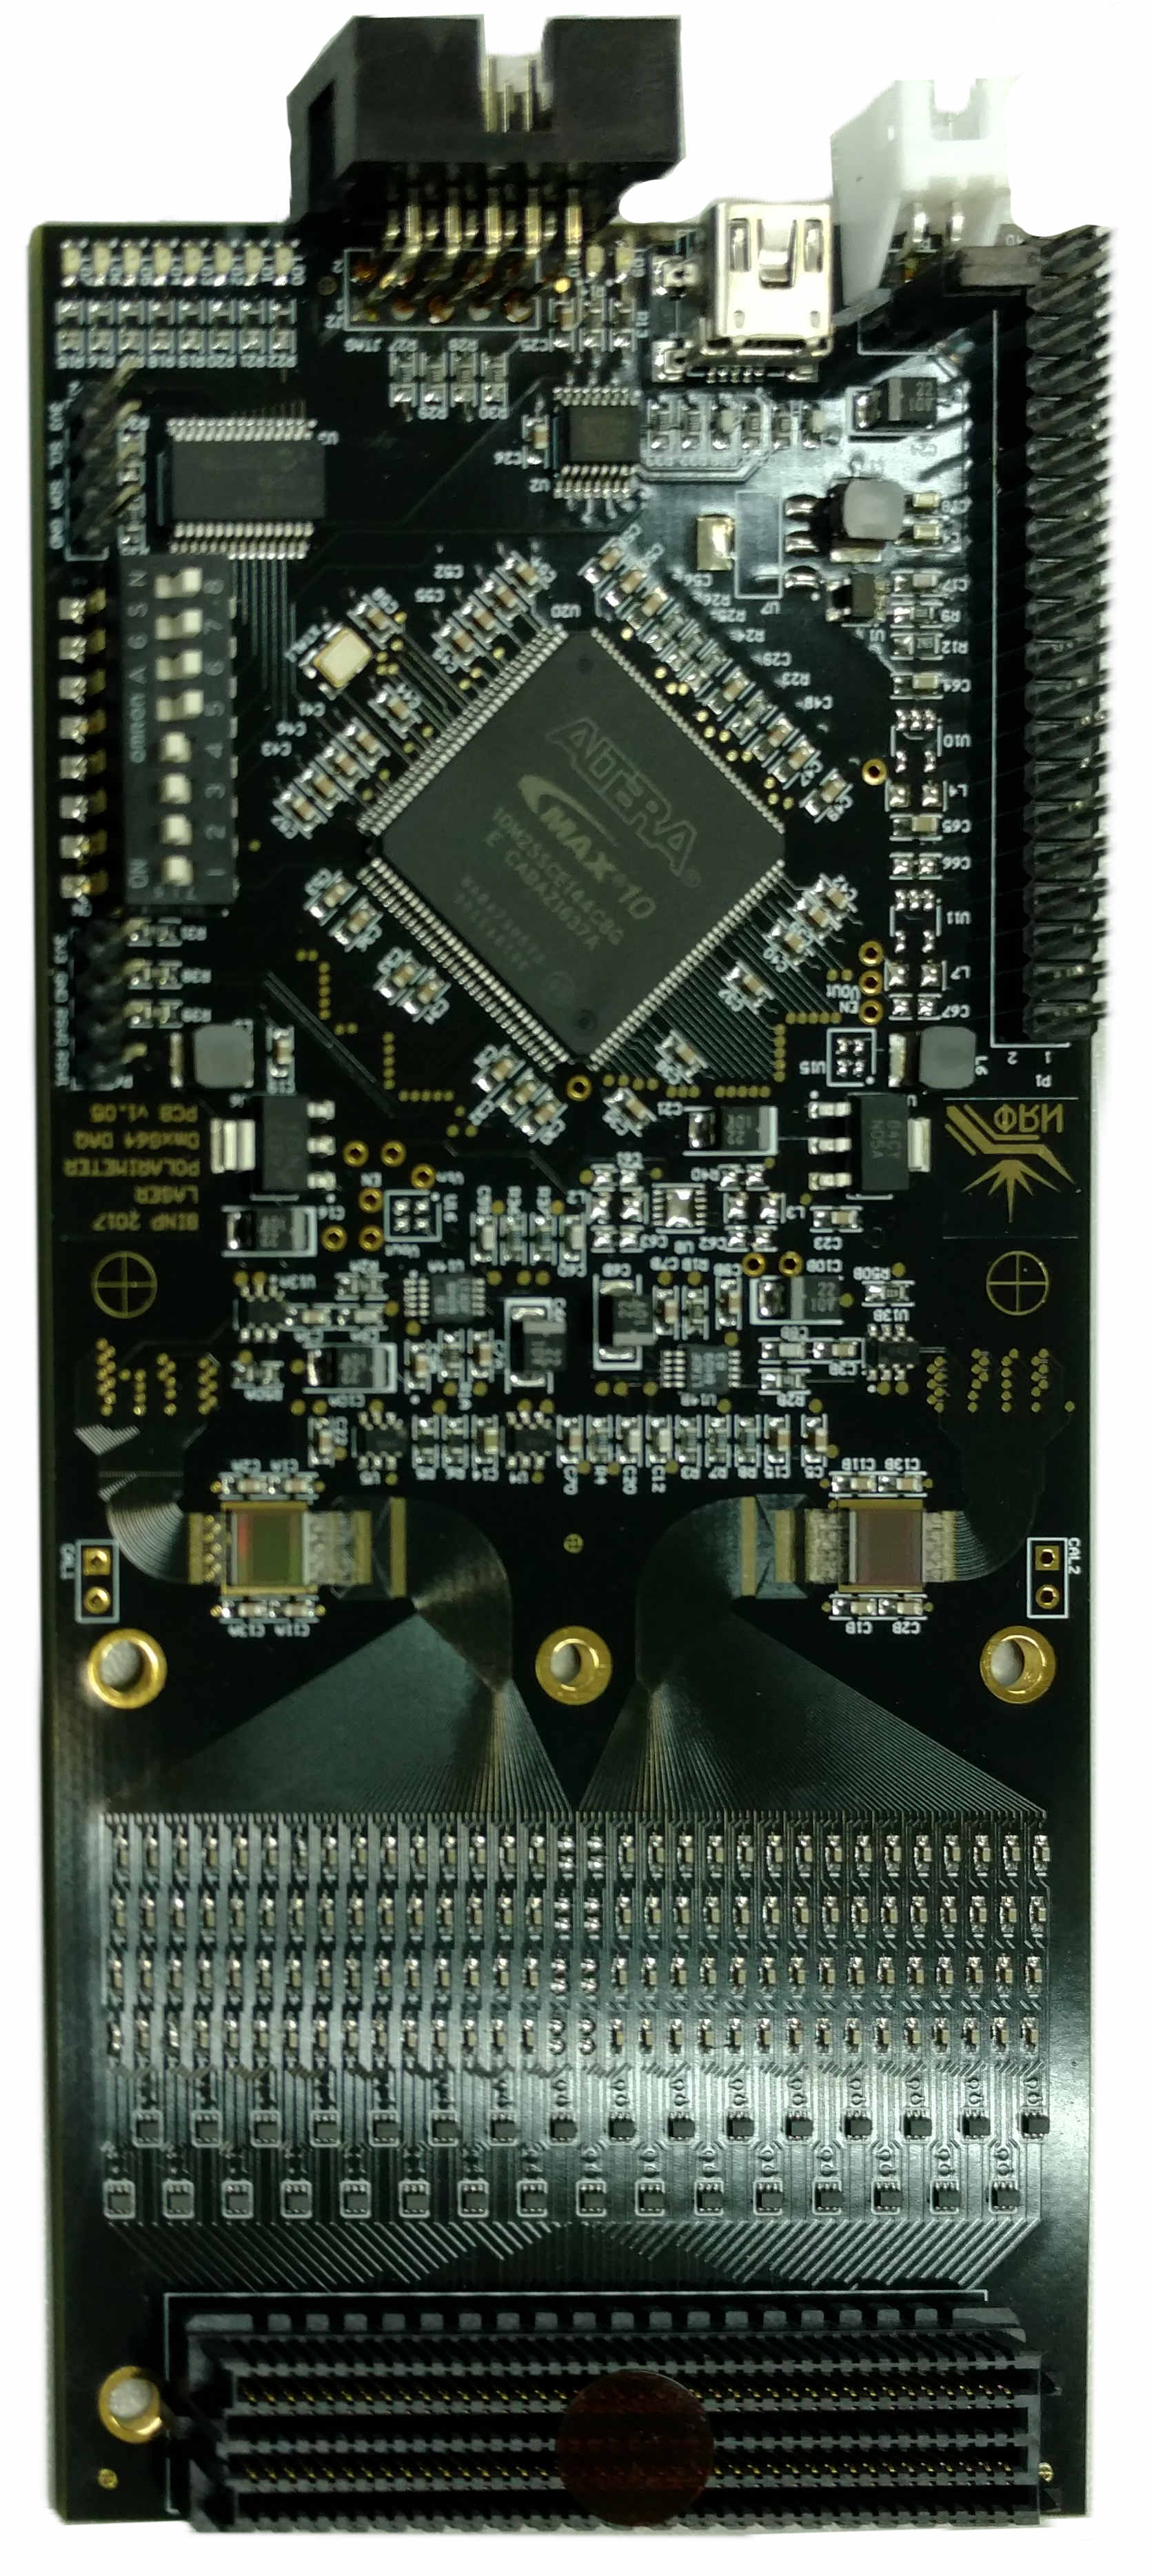
\includegraphics[width=0.5\linewidth]{Readout_board.jpg}
	\end{minipage}
\end{columns}
\end{frame}

\begin{frame}
\frametitle{Механизм газового усиления}
\begin{minipage}[h]{0.49\linewidth}
	\includegraphics[width=1\linewidth]{Gas_discharge_gr.png}
\end{minipage}
\begin{minipage}[h]{0.49\linewidth}
	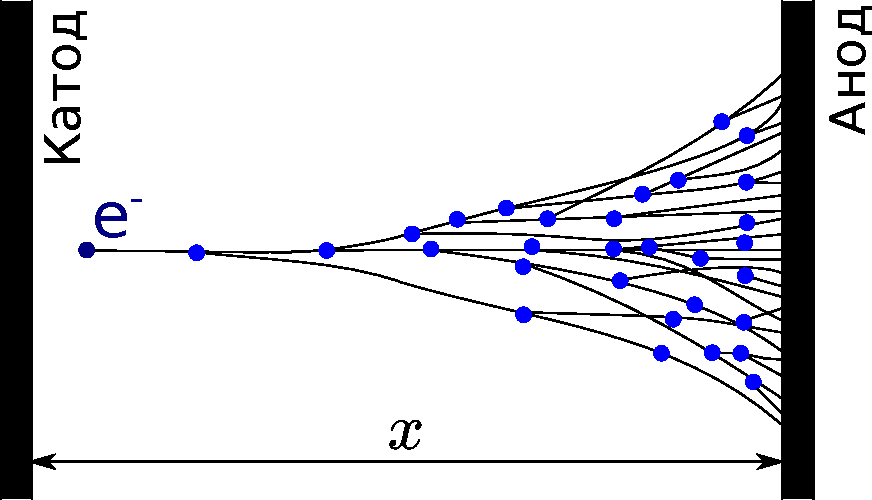
\includegraphics[width=1\linewidth]{Electron_avalanche.pdf}
	\newline
	\newline \footnotesize{Условие возникновения: $E_e \gtrsim W_I$}
	\newline (Не путать $W_I$ c $I$)
\end{minipage}
\end{frame}

\begin{frame}[t]
\frametitle{Коэффициент газового усиления}
\vspace{0pt}
\begin{columns}
\column{0.5\textwidth}
\begin{minipage}[t][1\textheight]{\linewidth}
	\small{
		\vspace*{30pt}
		\begin{itemize}
			\item Количество первичной ионизации: $n_{0} = \cfrac{\Delta E}{W_I}$
			\item $n_{tot} = n_{0} e^{\alpha x}$
			\item $\displaystyle n_{tr} = n_{tot} \epsilon = n_{0}\color{red}{K}$
		\end{itemize}
		Для GEM прозрачность можно определить как: 
		$\epsilon = \cfrac{\pi d^2}{2\sqrt{3}p^2}\cfrac{E_{ext}}{E_{hole}}$
	}
\end{minipage}%
\column{0.5\linewidth}
\begin{minipage}[t][1\textheight]{\linewidth}
	\vspace*{40pt}
	\center 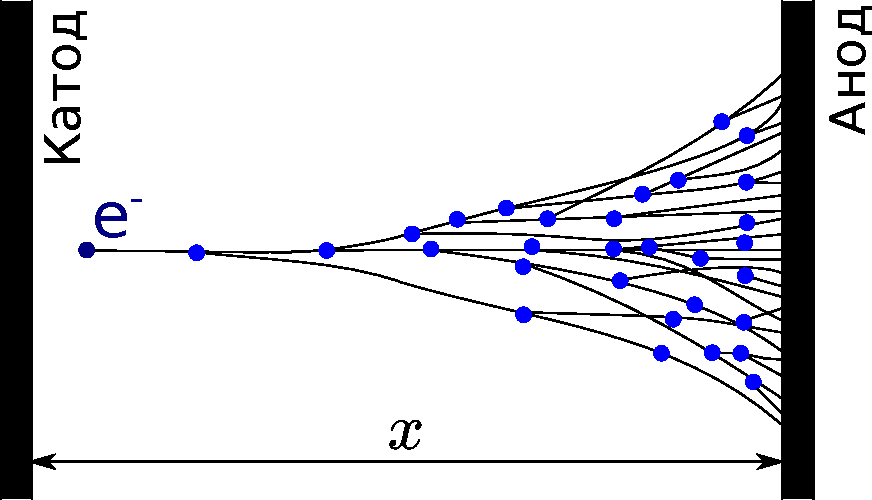
\includegraphics[width=0.9\linewidth]{Electron_avalanche.pdf}
\end{minipage}%
\end{columns}
\end{frame}

\begin{frame}[t]
\frametitle{Измерение коэффициента усиления GEM}
\vspace{0pt}
\begin{columns}
\column{0.5\textwidth}
\begin{minipage}[t][1\textheight]{\linewidth}
\small{\begin{itemize}
		\item $Sr-90$ в качестве источника первичной ионизации
		\item Регистрировались кластеры в центральной области под источником
		\item Знаем  $N_{e^-}$ первичной ионизации $\Rightarrow Q_{0}$ 
		\item Измерив $\langle Q\rangle$ кластера, можем найти $K$
\end{itemize}}
\end{minipage}%
\column{0.5\linewidth}
\begin{minipage}[t][1\textheight]{\linewidth}
\vspace*{20pt}
\center 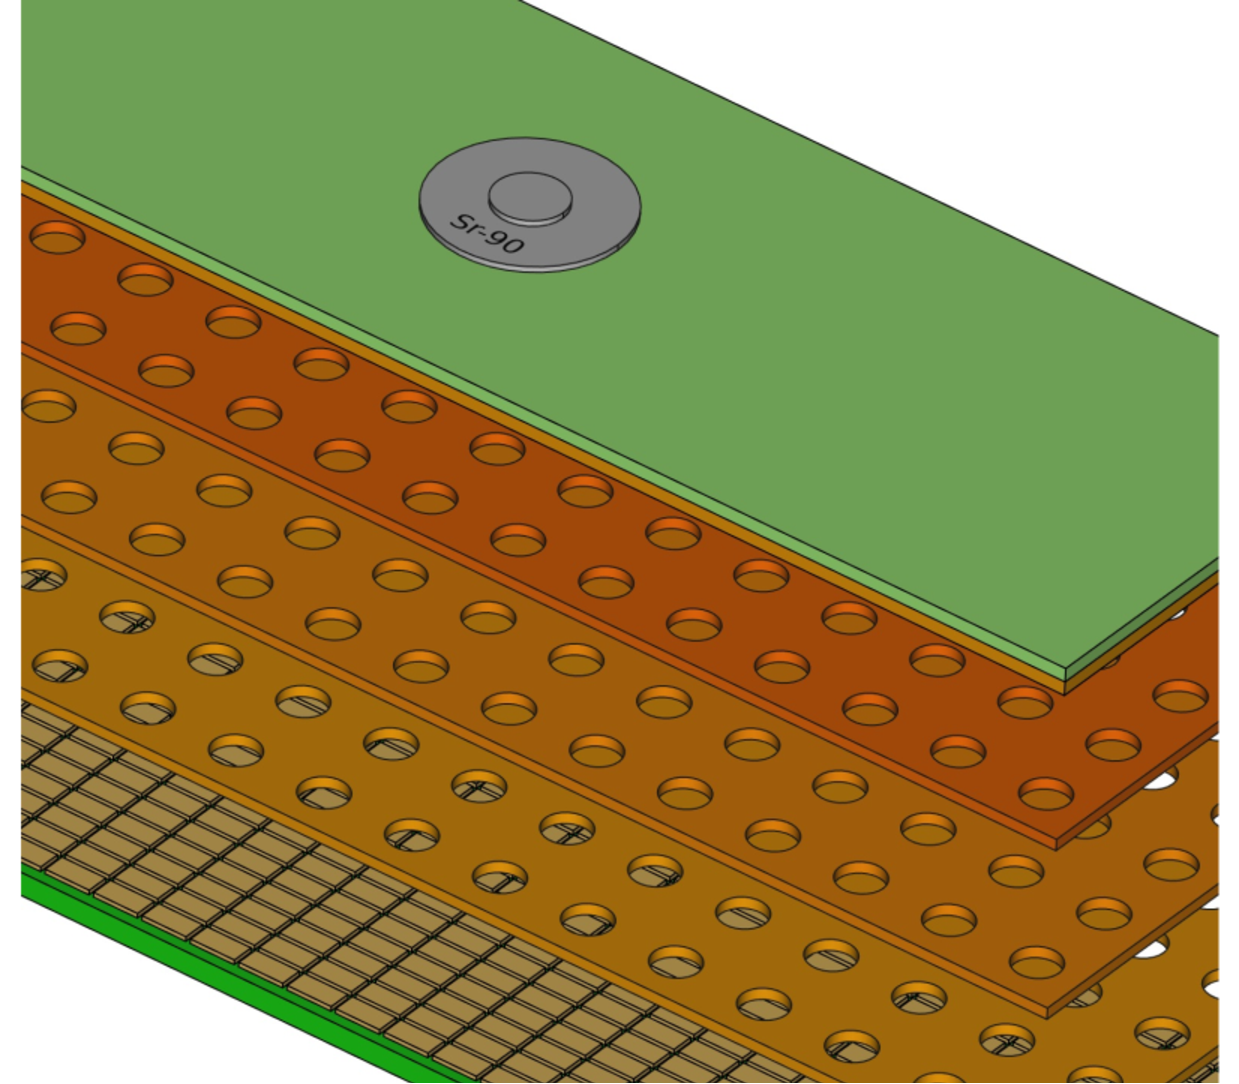
\includegraphics[width=0.9\linewidth]{GEM_Sr_source.pdf}

\end{minipage}%
\end{columns}
\end{frame}

\begin{frame}[t]
\frametitle{Сигнальное событие}

\begin{columns}
	\begin{column}{0.45\paperwidth}
		\small{
		\begin{itemize}
			\item Сигналы отдельных частиц(кластеры) \tikz[na] \coordinate (sig);
			\item Кадр со смещенным ``нулём'' \tikz[na] \coordinate (frame);
			\item Различный средний уровень каждого чипа \tikz[na] \coordinate (level);
		\end{itemize}
		}
	\end{column}
	\begin{column}{0.45\paperwidth}
		\vspace*{10pt}
		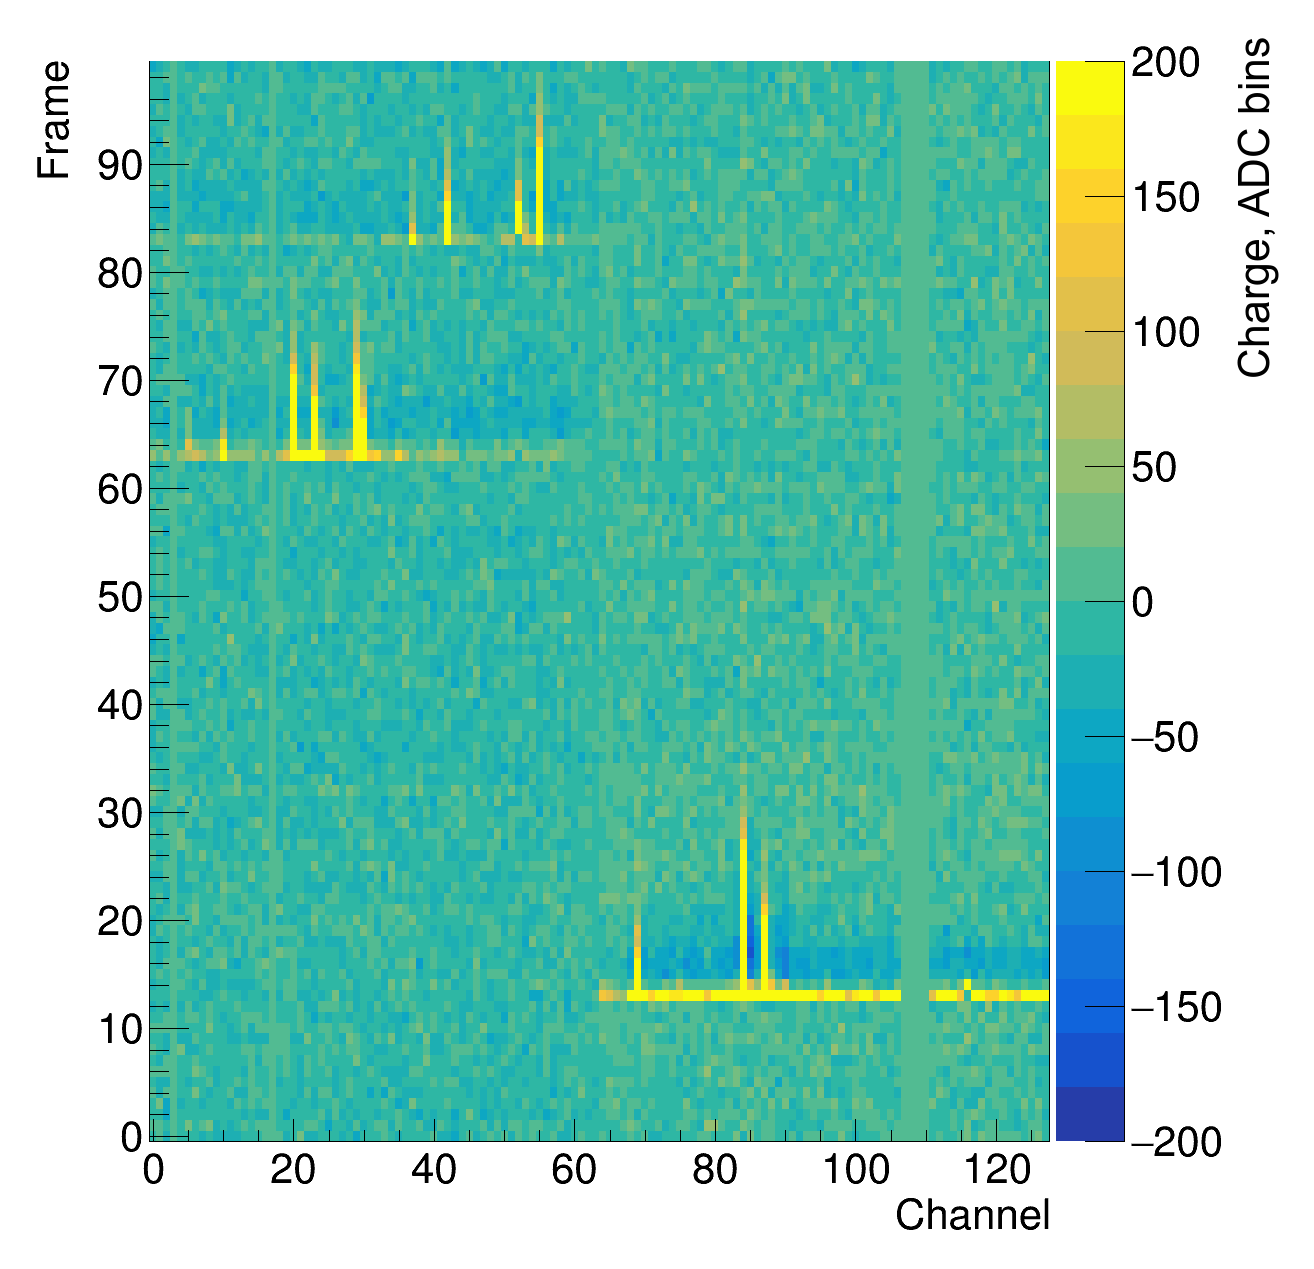
\includegraphics[width=1\textwidth]{Signal.png}
		\begin{tikzpicture}[overlay]
		%\draw[step=1.0,black,thin] (0,0) grid (7,7);
		\draw[->,red,thick] (-1,4.2) -- (2,5.3);
		\draw[->,red,thick] (-1,4.2) -- (1.5,4.5);
		\draw[->,red,thick] (-1,4.2) -- (3.3,2.3);
		\draw[->,blue,thick] (-1,3) -- (3,1.8);
		\draw[->,green,thick] (-1,1.7) -- (4,1.5);
		\draw[->,green,thick] (-1,1.7) -- (1.5,1.5);
		\end{tikzpicture}
	\end{column}
\end{columns}
\end{frame}

\begin{frame}[t]
\frametitle{Физический сдвиг нулевого уровня в кадре}
\vspace{0pt}
\begin{columns}
	\column{0.5\textwidth}
	\begin{minipage}[t][1\textheight]{\linewidth}
		\small{\begin{itemize}
				\item Есть кадр со смещенным нулевым уровнем
				\item 1-8 сигнальных каналов/60
				\item $\langle Q_{noise}\rangle \neq 0 $
				\item \textbf{Проблема:} как при вычислении среднего не учитывать сигнальные события?
		\end{itemize}}
	\end{minipage}%
	\column{0.5\linewidth}
	\begin{minipage}[t][1\textheight]{\linewidth}
		%\vspace*{40pt}
		\hspace*{5pt}
		\centering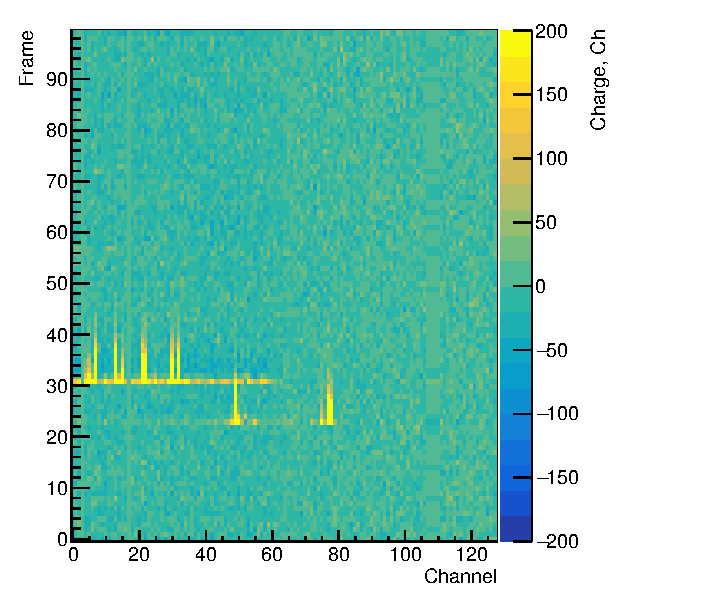
\includegraphics[width=1.05\linewidth]{median_monitor.pdf}
	
		
	\end{minipage}%
\end{columns}
\end{frame}

\begin{frame}[t]
\frametitle{Коррекция нулевого уровня в кадре}
\vspace{0pt}
\begin{columns}
	\column{0.5\textwidth}
	\begin{minipage}[t][1\textheight]{\linewidth}
		\vspace{30pt}
		\small{
		\textbf{Решение:} медианный алгоритм
		\begin{itemize}
				\item Нахождение медианного значения заряда по кадру
				\item $Q(Ch) = Q_{0}(Ch)- median$
		\end{itemize}}
	\end{minipage}%
	\column{0.5\linewidth}
	\begin{minipage}[t][1\textheight]{\linewidth}
		\vspace*{10pt}
		\centering 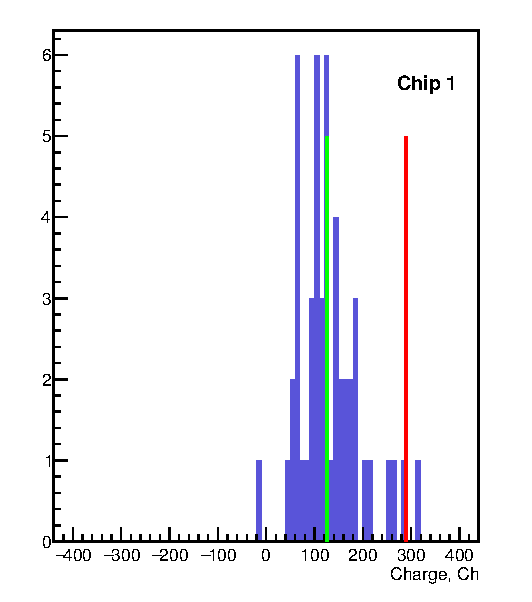
\includegraphics[ width=0.9\linewidth]{median_hist_zoomed.pdf}
	\end{minipage}%
\end{columns}
\end{frame}

\begin{frame}[t]
\frametitle{Результат применения алгоритма}
\vspace{0pt}
		\centering 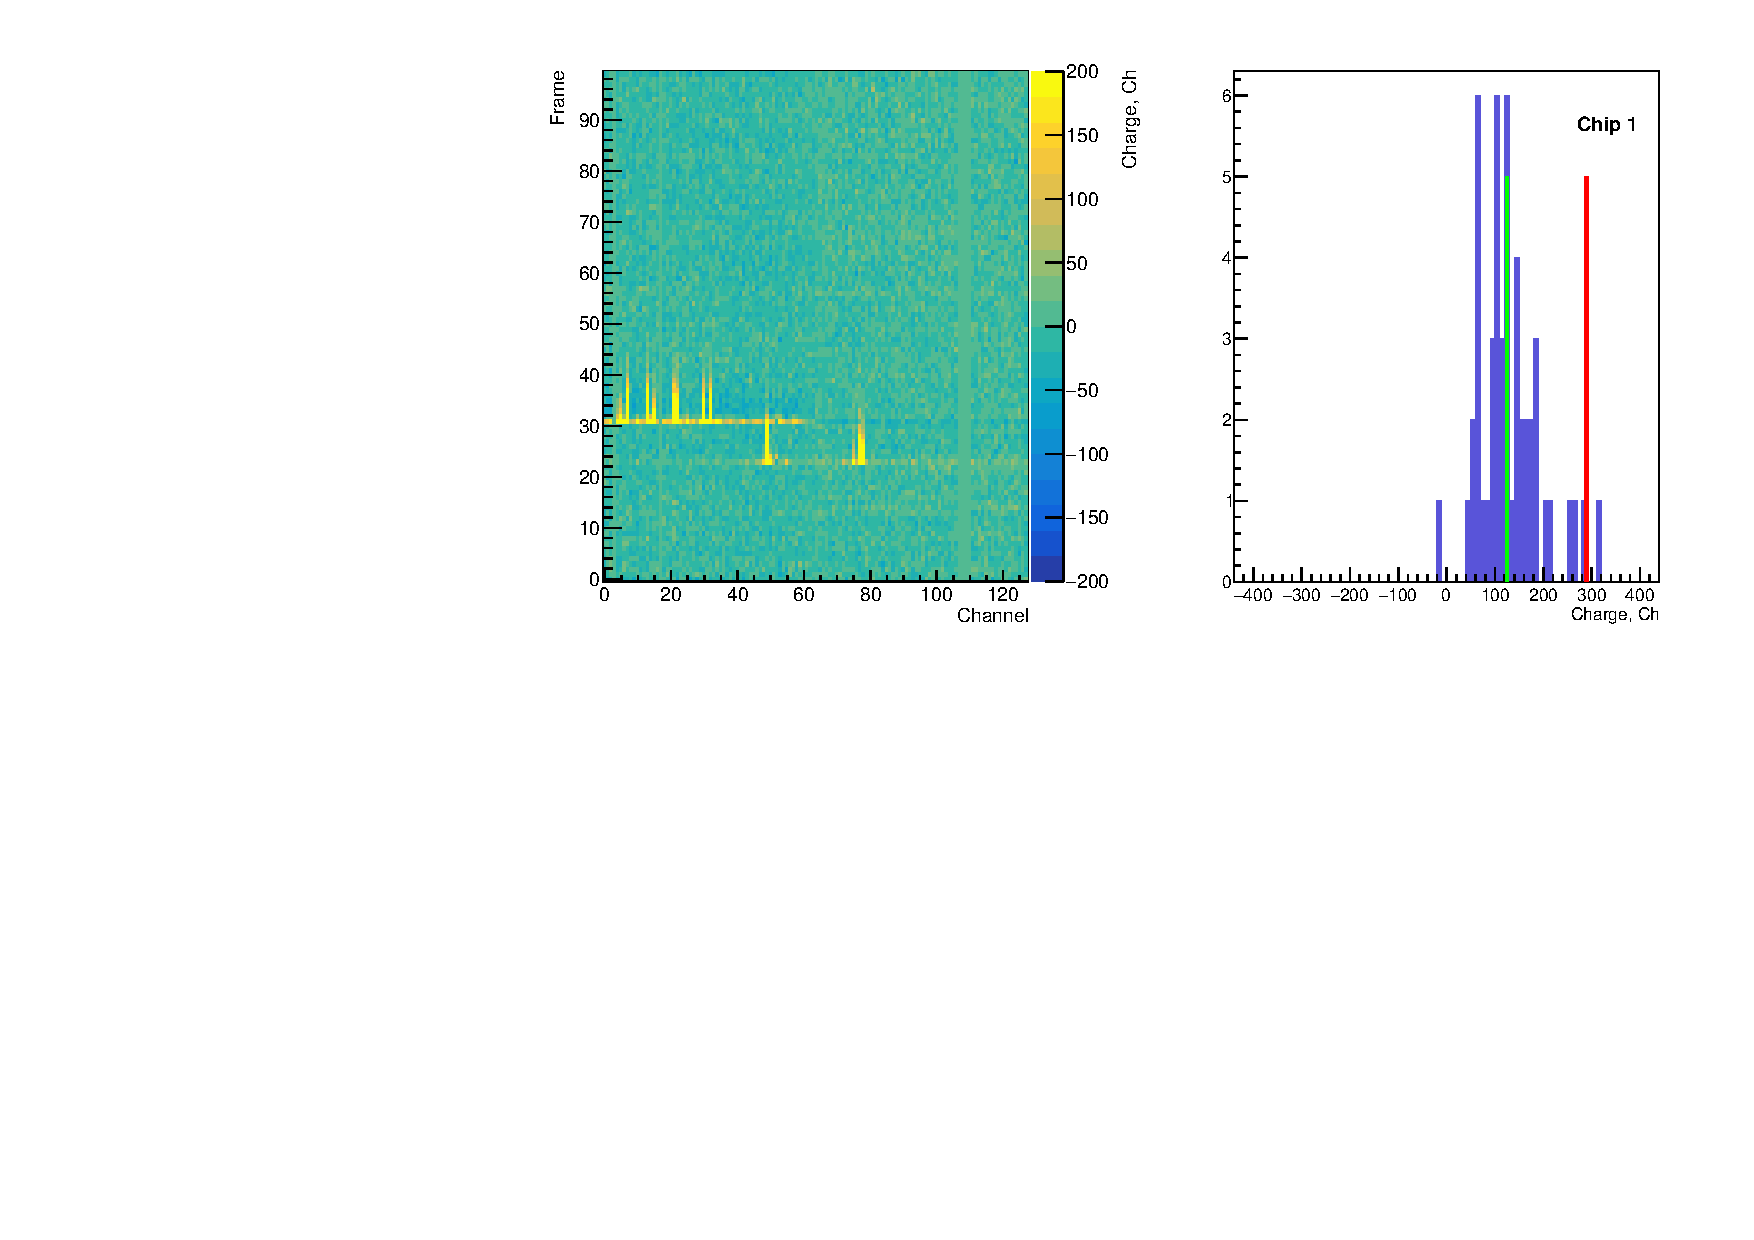
\includegraphics[height=0.4\textheight, width=0.7\linewidth]{median_hist_unbiased.pdf}
		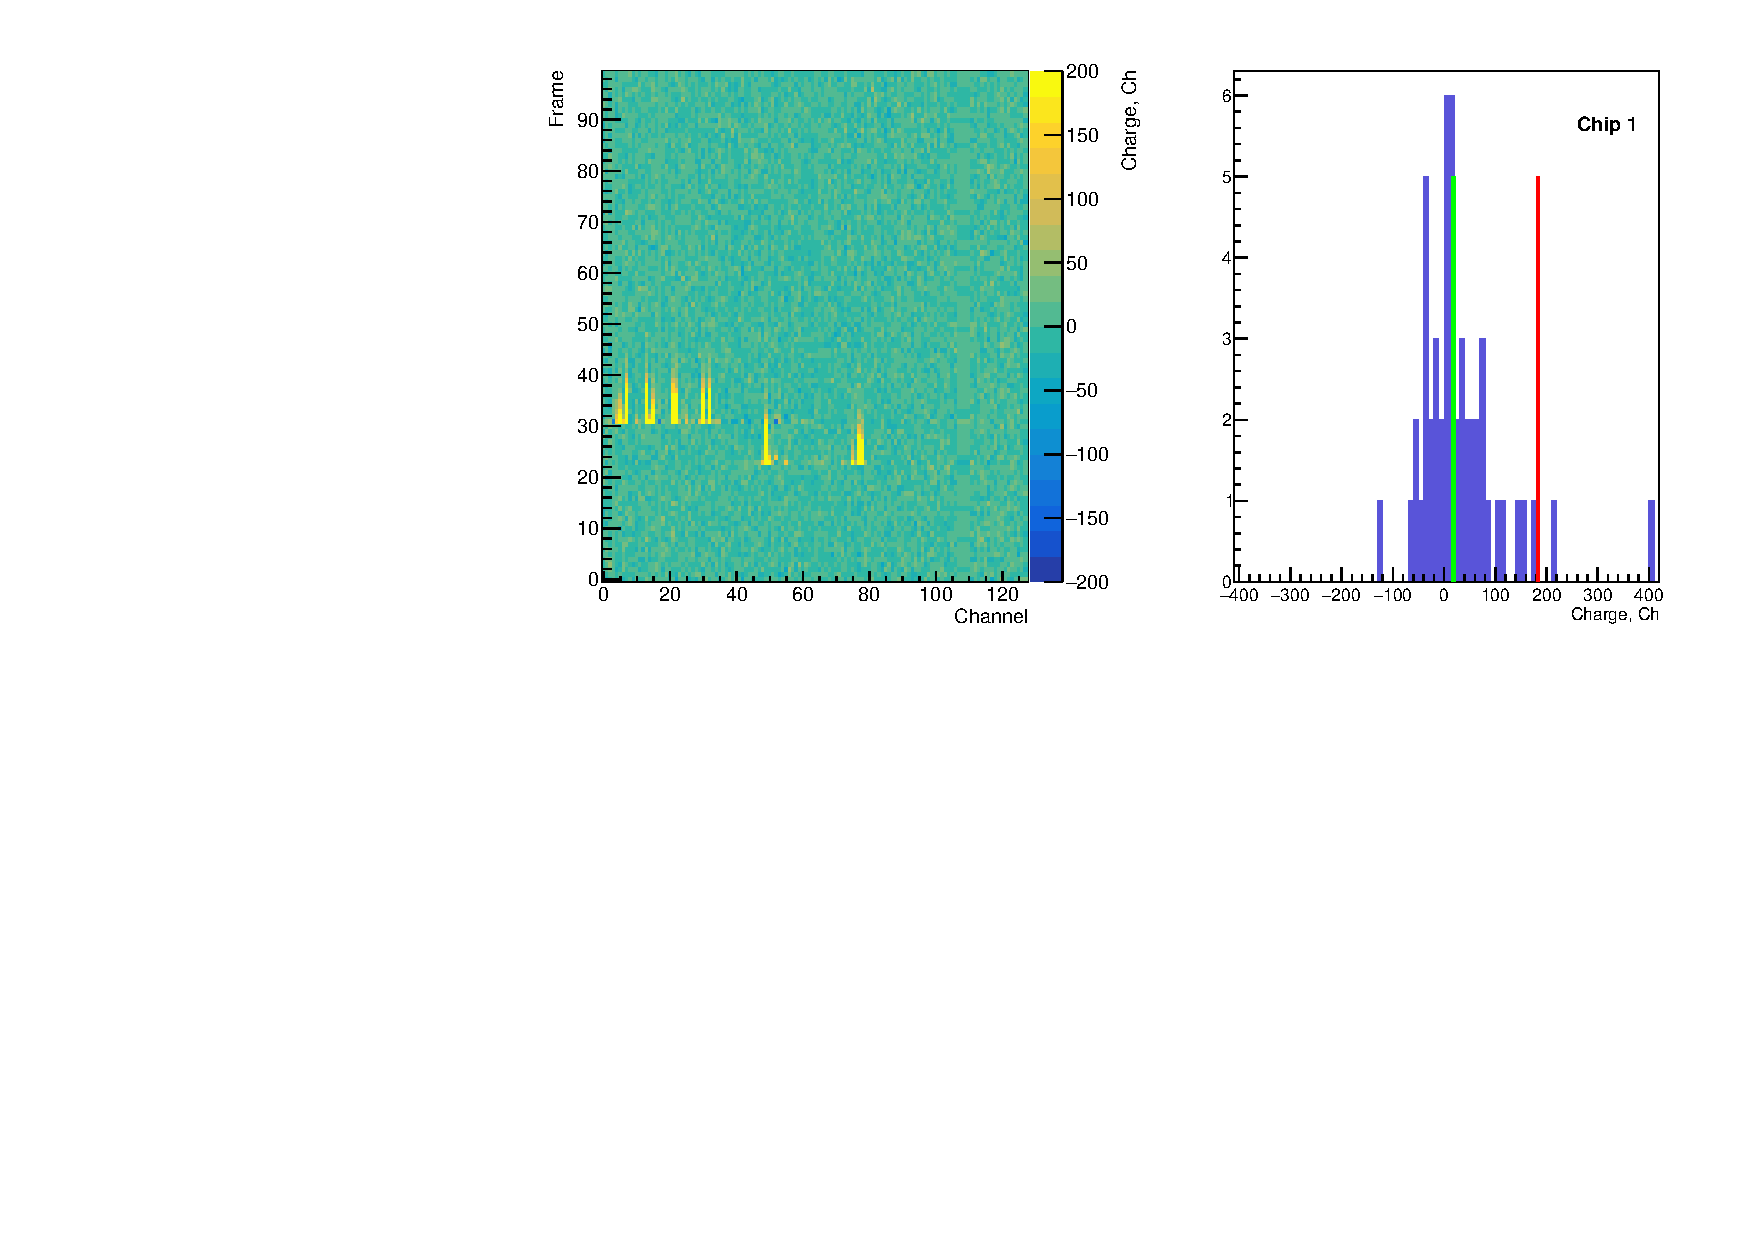
\includegraphics[height=0.4\textheight,width=0.7\linewidth]{median_hist_biased.pdf}
\end{frame}

\begin{frame}[t]
\frametitle{Измерение коэффициента усиления (обработка данных)}
\vspace{0pt}
\begin{columns}
	\column{0.5\textwidth}
	\begin{minipage}[t][1\textheight]{\linewidth}
		\small{\begin{itemize}
				\item Сигналы с соседних каналов $\rightarrow$ кластер
				\item $\Sigma Q_{sig}$ для кластера
				\item Распределение по $Q_{sig}$
				\item MPV $\rightarrow \langle Q_{sig} \rangle$
				\item $\displaystyle K = \cfrac{\langle Q_{sig} \rangle}{n_{0}e^{-}}$
		\end{itemize}}
	\end{minipage}%
	\column{0.5\linewidth}
	\begin{minipage}[t][1\textheight]{\linewidth}
		\centering 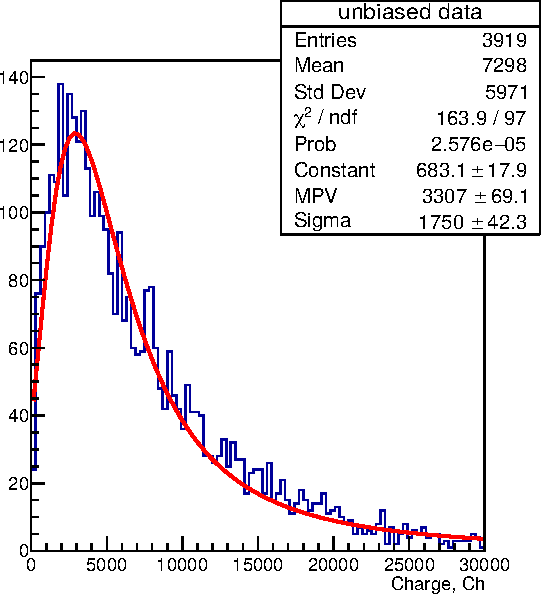
\includegraphics[ width=0.9\linewidth]{Cluster_ch_hist_unbiased.pdf}
	\end{minipage}%
\end{columns}
\end{frame}

\begin{frame}[t]
\frametitle{Зависимость коэффициента усиления от напряжения}
\vspace*{10pt}
\centering 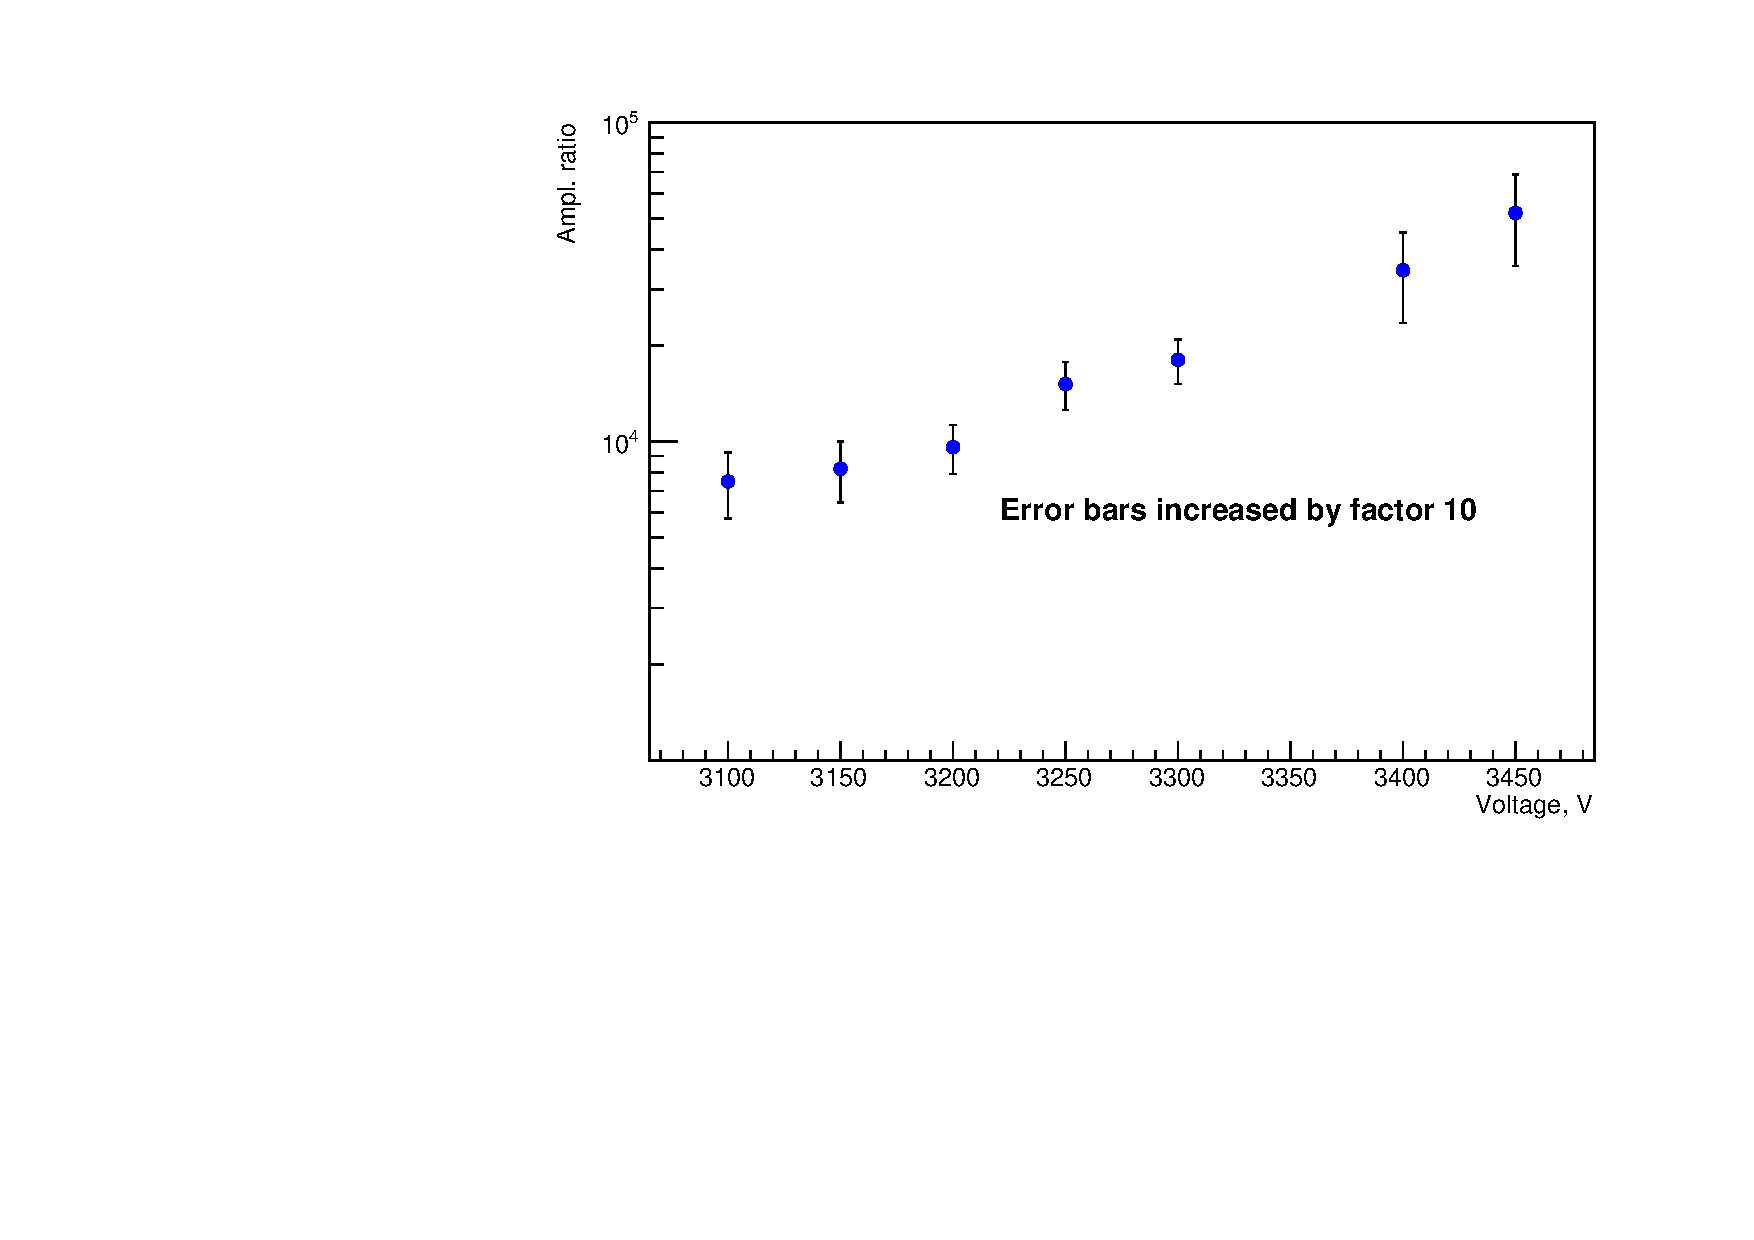
\includegraphics[ width=0.75\linewidth]{Ampl_gr_log.pdf}
\end{frame}
\begin{frame}[t]
\frametitle{Анализ полученных результатов}
\begin{columns}
	\column{0.5\textwidth}
	\begin{minipage}[t][1\textheight]{\linewidth}
		\small{\begin{itemize}
				\item Максимальный $K \approx 52000$
				\item При $K < 10000$ сигнал под шумами 
				\item Экспоненциальный рост K c увеличением напряжения питания
		\end{itemize}%ы
		Такое поведение K характерно для GEM, что является показателем правильной работы усиливающей структуры детектора}
	\end{minipage}%
	\column{0.5\linewidth}
	\begin{minipage}[t][1\textheight]{\linewidth}
		\vspace*{30pt}
		\center 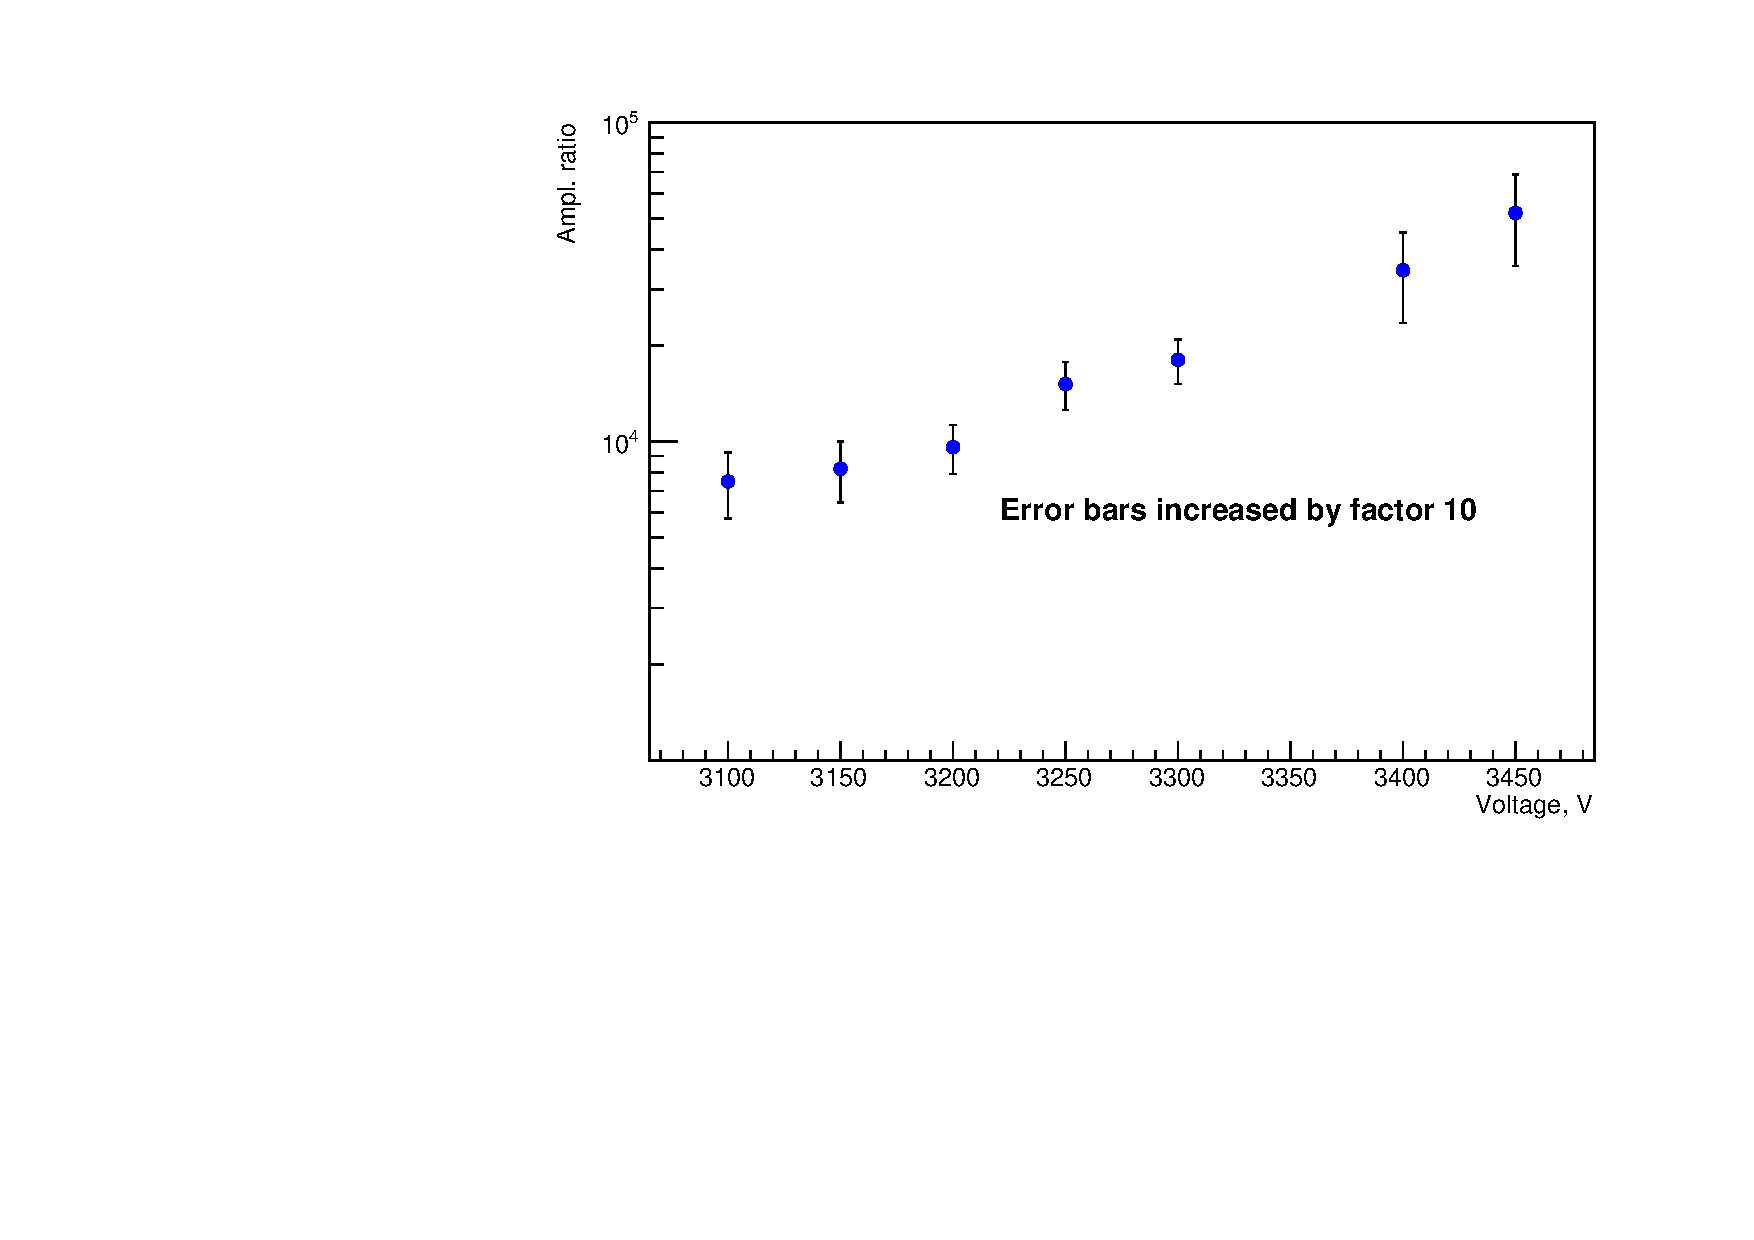
\includegraphics[ width=1\linewidth]{Ampl_gr_log.pdf}
	\end{minipage}%
\end{columns}
\end{frame}
\begin{frame}[t]
\frametitle{Заключение}
\begin{itemize}
	\item Разрабатывается прототип детектора для установки <<Лазерный поляриметр>>
	\item Уже получены данные об уровне шумов: $\sigma_{n} \approx 5700 e^{-}$
	\item и коэффициенте усиления GEM: $K_{max} \approx 52000$
	\item \color{calmRed} {Необходимо исследование пространственного разрешения и эффективности регистрации на выведенном пучке}
\end{itemize}
\end{frame}
\begin{frame}
\begin{center}
Спасибо за внимание!
\end{center}
\end{frame}
\backupbegin
\begin{frame}
\frametitle{Backup: пьедесталы АЦП}
\begin{center}
	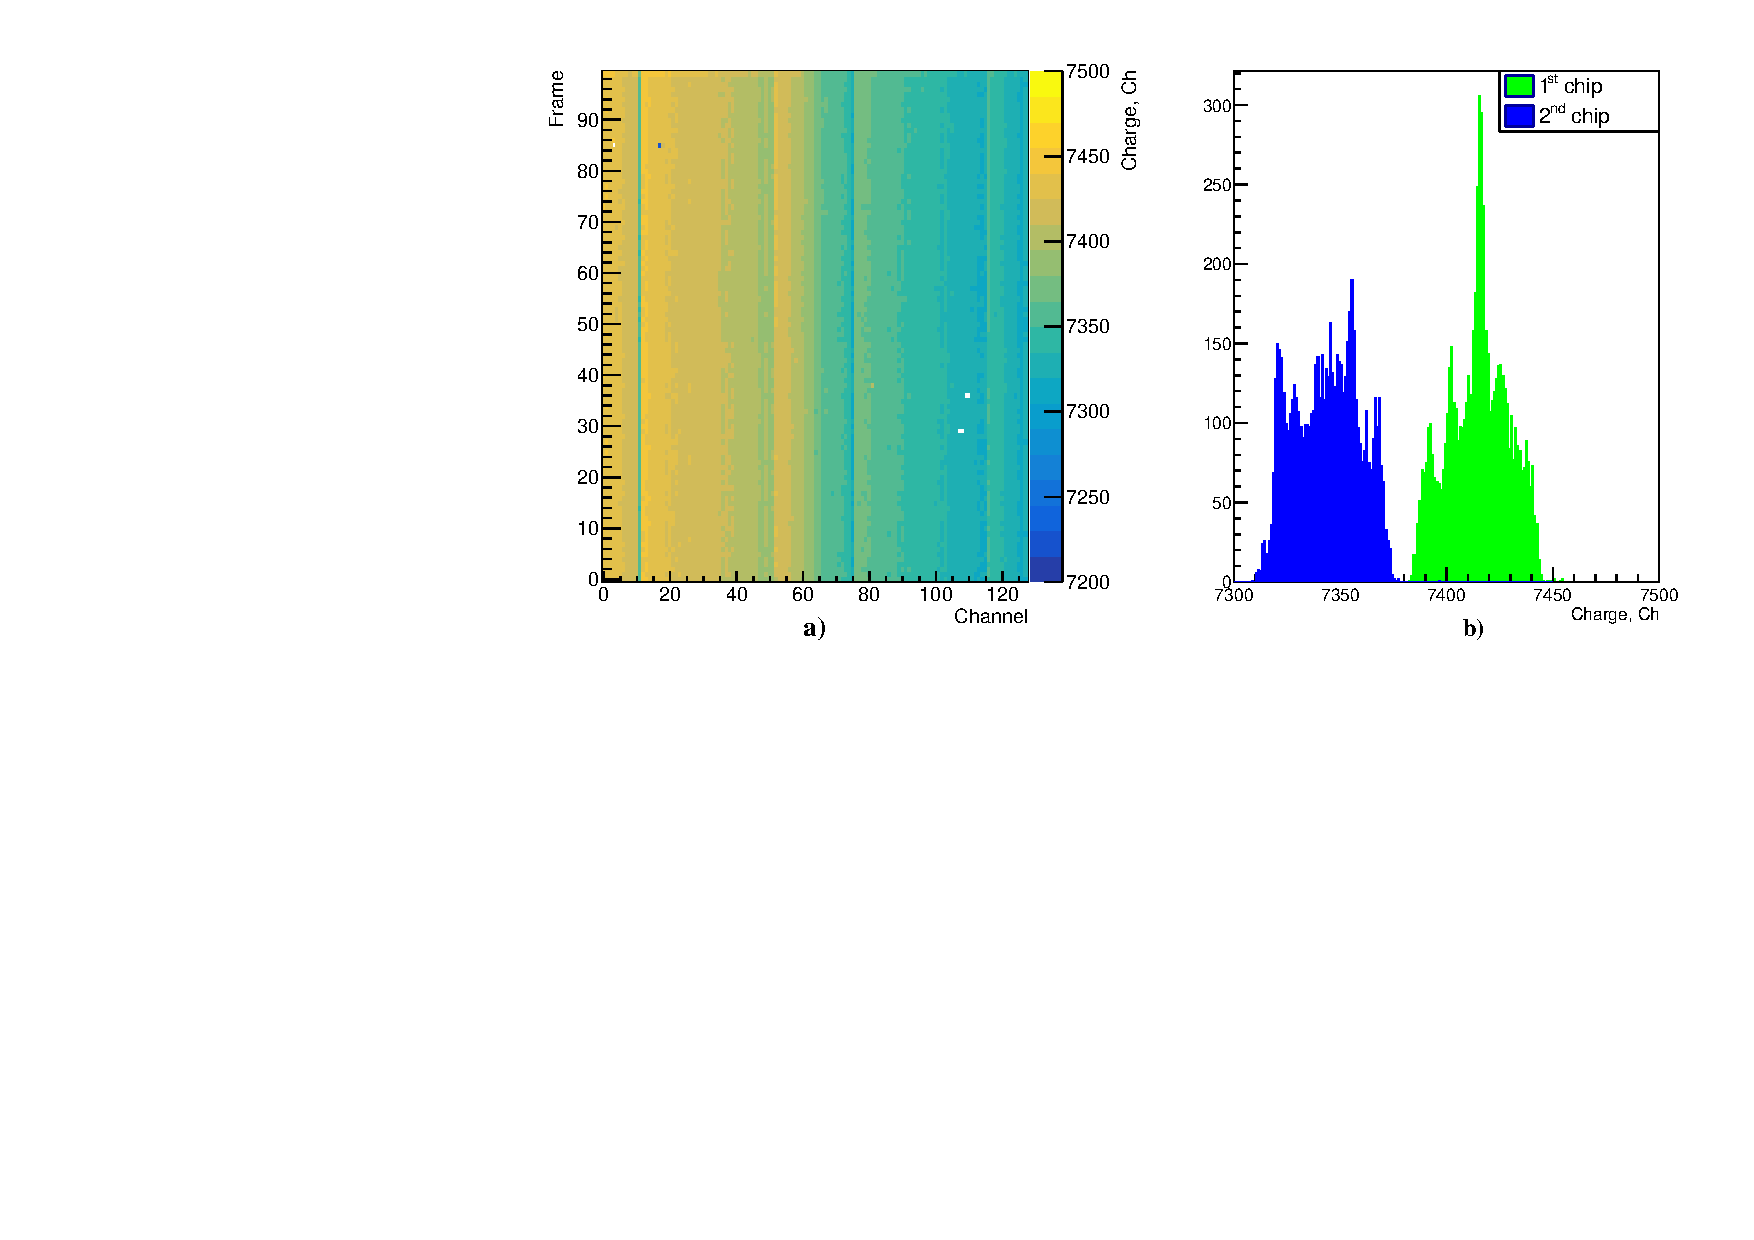
\includegraphics[ width=0.9\linewidth]{pedestal_map.pdf}
\end{center}
\end{frame}

%\begin{frame}
%\frametitle{Backup: план выполнения работ}
%\begin{center}
%	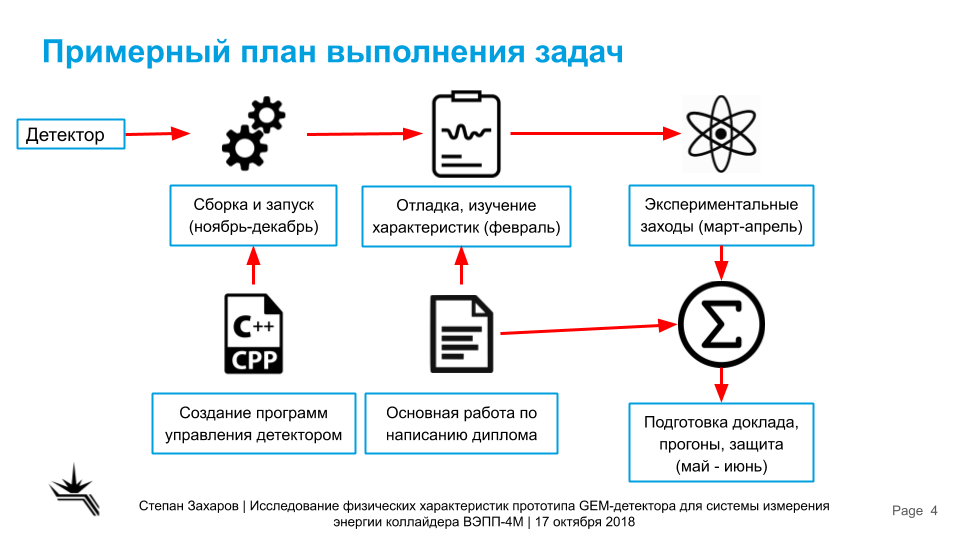
\includegraphics[ width=0.9\linewidth]{schedule.png}
%\end{center}
%\end{frame}
\begin{frame}[t]
\frametitle{Backup: Потери энергии в детекторе}
Для $2.2~\MeV~e^{-}$:
\newline
\newline $\kappa = \cfrac{dE/dx_{rad}}{dE/dx_{ion}}= \cfrac{ Z E[\MeV] }{600}.$
\newline 
\newline Используем Ar: $E_{crit} = 33.3~\MeV > 2.2 \MeV~\Rightarrow$ потери ионизационные.
\newline
\newline $X_0(Ar)=117$м,
\newline
\newline $\cfrac{dE}{dx} = \cfrac{2\pi N_0 e^4 Z\rho}{m_e c^2 \beta^2 A}\biggl[ln\cfrac{ m_ec^2E}{I^2}\cfrac{\beta^2}{2(1-\beta^2)} + f_{corr}(\beta)\biggr]$

\end{frame}

\begin{frame}[t]
\frametitle{Backup: Влияние медианного алгоритма}
\vspace*{10pt}
\centering 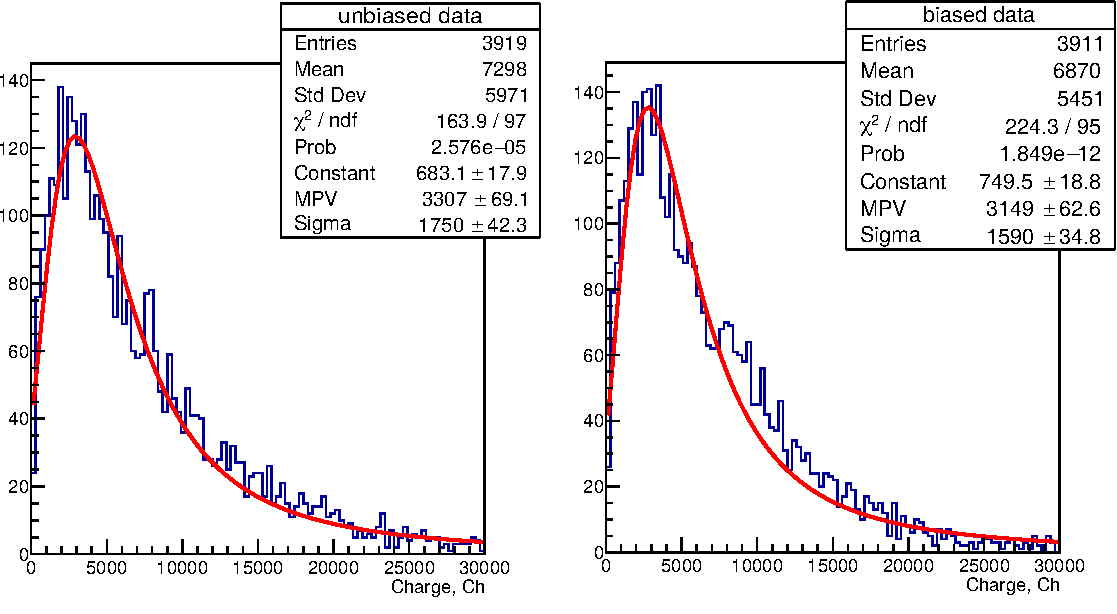
\includegraphics[ width=0.9\linewidth]{Cluster_ch_hist.pdf}
\end{frame}
\backupend
\end{document} 